% Copyright 2004 by Till Tantau <tantau@users.sourceforge.net>.
%
% In principle, this file can be redistributed and/or modified under
% the terms of the GNU Public License, version 2.
%
% However, this file is supposed to be a template to be modified
% for your own needs. For this reason, if you use this file as a
% template and not specifically distribute it as part of a another
% package/program, I grant the extra permission to freely copy and
% modify this file as you see fit and even to delete this copyright
% notice. 

\documentclass[xcolor=dvipsnames]{beamer}
\usepackage{bibentry}
\setbeamertemplate{bibliography item}{\insertbiblabel}
\usepackage{cancel}
\usepackage{amsmath} 
\usepackage{mathtools}
\newcommand{\norm}[1]{\left\lVert #1 \right\rVert}
% Command for round parenthesis
\newcommand{\roundP}[1]{\left( #1 \right)}
% Command for poisson brackets
\newcommand{\poisson}[2]{\left\lbrace #1, #2 \right\rbrace}

\usepackage{varwidth}
\usepackage{lipsum}
\usepackage{color}
\usepackage{todonotes}
\definecolor{dgray}{gray}{0.30}
\definecolor{uyellow}{RGB}{253,241,0}

\usepackage[utf8]{inputenc}
\usepackage{graphicx}
\usepackage{epstopdf}
\usepackage[english]{babel}
\usepackage{hyperref}
\usepackage{datenumber}
\usepackage{todonotes}
\usepackage{mathtools}
\usepackage{amsmath}
\usepackage{amssymb}
\usepackage{amsthm}
\usepackage[caption=true]{subfig}

\newtheorem*{thm}{Theorem}
\newcommand{\fmunu}{F^{\mu\nu}}
\newcommand{\E}{\vec{E}}
\newcommand{\B}{\vec{B}}
\newcommand{\rot}{\nabla\times}
\newcommand{\dive}{\nabla\cdot}
\newcommand{\tmunu}{T^{\mu\nu}}
\newcommand{\levichi}{\epsilon_{\mu\nu\sigma\gamma}}
\newcommand{\dete}{\textrm{det}}
\newcommand{\lna}{\textrm{ln}}
\newcommand{\Tr}{\textrm{Tr}}
\newcommand{\seno}{\textrm{sin}}

\makeatletter
\newcommand{\pushright}[1]{\ifmeasuring@#1\else\omit\hfill$\displaystyle#1$\fi\ignorespaces}
\newcommand{\pushleft}[1]{\ifmeasuring@#1\else\omit$\displaystyle#1$\hfill\fi\ignorespaces}
\makeatother



% There are many different themes available for Beamer. A comprehensive list with examples is given here:
% http://deic.uab.es/~iblanes/beamer_gallery/index_by_theme.html
%\usetheme{AnnArbor}
%\usetheme{Antibes}
%\usetheme{Bergen}
%\usetheme{Berkeley}
%\usetheme{Berlin}
%\usetheme{Boadilla}
%\usetheme{boxes}
%\usetheme{CambridgeUS}
\usetheme{Copenhagen}
%\usetheme{Darmstadt}
%\usetheme{default}
%\usetheme{Frankfurt}
%\usetheme{Goettingen}
%\usetheme{Hannover}
%\usetheme{Ilmenau}
%\usetheme{JuanLesPins}
%\usetheme{Luebeck}
%\usetheme{Madrid}
%\usetheme{Malmoe}
%\usetheme{Marburg}
%\usetheme{Montpellier}
%\usetheme{PaloAlto}
%\usetheme{Pittsburgh}
%\usetheme{Rochester}
%\usetheme{Singapore}
%\usetheme{Szeged}
%\usetheme{Warsaw}
%\usecolortheme{seagull}
%\usetheme{Malmoe} 

\setbeamercolor{frametitle}{fg=Black,bg=Blue!60}
\setbeamercolor{section in head/foot}{bg=Blue, fg=Black}
\setbeamercolor{author in head/foot}{bg=blue, fg=Black} 
\setbeamercolor{date in head/foot}{fg=blue} 
\setbeamercolor{institute in head/foot}{fg=Black}
\usecolortheme[named=Black]{structure}
\setbeamerfont{footnote}{size=\footnotesize}

\setbeamertemplate{}[page number] % To replace the footer line in all slides with a simple slide count uncomment this line
 
\title{\textbf{The Expected Shape of the Milky Way's Dark Matter Halos }}

% A subtitle is optional and this may be deleted
%\subtitle{Optional Subtitle}

\author{Jesus Prada}
% - Give the names in the same order as the appear in the paper.
% - Use the \inst{?} command only if the authors have different affiliation.

\institute[{\color{Black} Universidad de los Andes}] % (optional, but mostly needed)
{
 \normalsize Advisors:\\
 PhD Jaime E. Forero-Romero \\ \small Universidad de los Andes, Departamento de Física\\
  \vspace{5mm}
 \normalsize PhD Volker Springel \\ \small  Heidelberg's Institute of Theoretical studies
}
% - Use the \inst command only if there are several affiliations.
% - Keep it simple, no one is interested in your street address.

\tiny
\date{ \footnotesize May, 2018}
% - Either use conference name or its abbreviation.
% - Not really informative to the audience, more for people (including yourself) who are reading the slides online
	

\subject{The Expected Shape of the Milky Way's Dark Matter Halo}
% This is only inserted into the PDF information catalog. Can be left out. 

% If you have a file called "university-logo-filename.xxx", where xxx  is a graphic format that can be processed by latex or pdflatex, resp., then you can add a logo as follows:
% \pgfdeclareimage[height=0.5cm]{university-logo}{university-logo-filename}
% \logo{\pgfuseimage{university-logo}}

% Delete this, if you do not want the table of contents to pop up at the beginning of each subsection:
%\AtBeginSubsection[] { \begin{frame}<beamer>{Outline} \tableofcontents[currentsection,currentsubsection] \end{frame}}

% Let's get started
\begin{document}

\begin{frame}
  \titlepage
\end{frame}
%--------------------------------------------
\begin{frame}{Outline}
 \tableofcontents
  % You might wish to add the option [pausesections]
\end{frame}
%------------------------------------------------
\section{Motivation}
\subsection{Evidences of Dark Matter (DM)}
\begin{frame}

\begin{columns}[c]

\begin{column}{.5\textwidth}
\begin{figure}
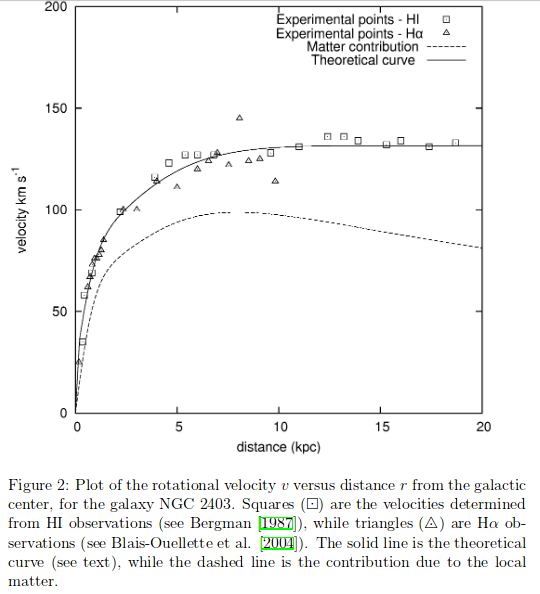
\includegraphics[width=1\linewidth]{./pics/RotationCurves.png}
\caption{\tiny arxiv:1111.5793}
\end{figure}
\end{column}

\begin{column}{.5\textwidth}
\centering
\begin{itemize}
\small
\item Rotation curves
\item Weak lensing
\item CMB
\item Large-scale structure of the universe
\item Modified gravity
\end{itemize}
\end{column}

\end{columns}

\end{frame}
%--------------------------------------------------------------------------------------
\subsection{DM density in our Milky Way (MW)}
\begin{frame}
\begin{itemize}
\small
\item We have not measured DM directly.
\item \textbf{DM density field} of an object is needed.
\item DM evidence is not that far: MW
\item MW is the only object of which we have tridimensional view from the interior.
\end{itemize}

\begin{figure}[c]
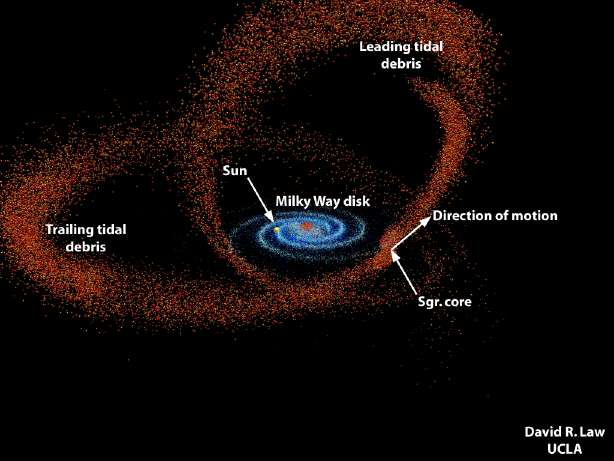
\includegraphics[width=0.5\linewidth]{./pics/Sagitarius.jpg}
\caption{\tiny Sagitarius stream. David Law}
\end{figure}

\end{frame}
%-----------------------------------------------------------------------------------------
\begin{frame}
\small
The DM density field is often reduced to a radial profile:

\begin{equation}
\rho(\vec{r}) \rightarrow \rho(r) = \frac{\delta_c \rho_{crit}}{\frac{r}{r_c}\left( 1 + \frac{r}{r_c}\right)},
\end{equation}

which is universal in a hierarchical model of formation \cite{Navarro1997}.\\~\\

Radial profiles omit angular dependence of density (\textbf{shape}).\\~\\

DM halos are not \textbf{spherical} but \textbf{triaxial} \cite{Allgood2006} (acretion)\\~\\

\begin{block}
{Why do we want to define a shape?}
Besides being a more complete characterization of density, it can keep memory of past events of formation.
\end{block}

\end{frame}
%---------------------------------------------------------------------------------------
\subsection{Observational constraints on MW's DM halo}
\begin{frame}

Some efforts for constraints on the MW's DM halo shape. \cite{Loebman2012,LawMajewski2010,Vera-Ciro2013,}

\begin{figure}[c]
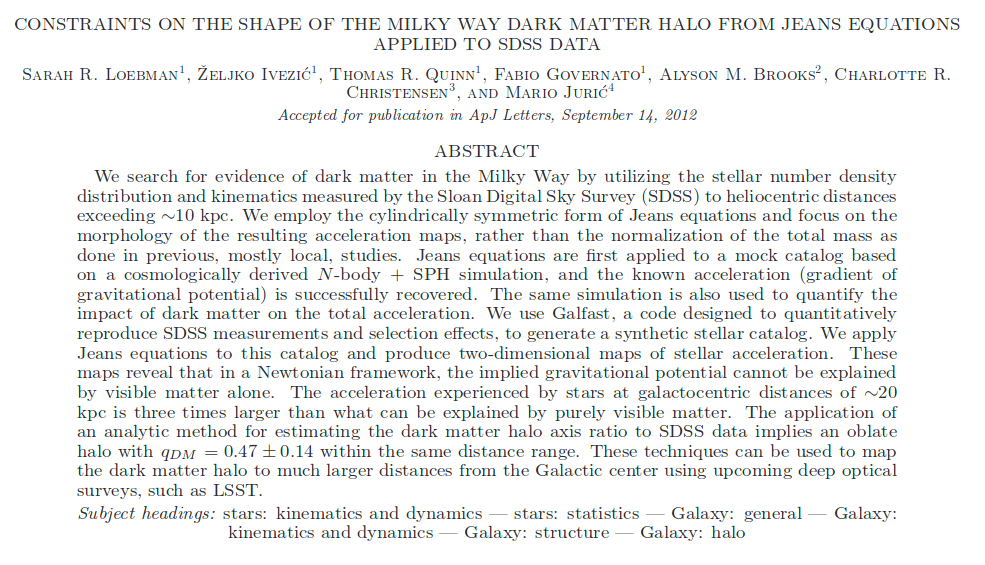
\includegraphics[width=1\linewidth]{./pics/loebmanJean.png}
\end{figure}


\end{frame}
%---------------------------------------------------------------------------------------
\begin{frame}

\begin{columns}[c]

\begin{column}{.5\textwidth}
\begin{figure}
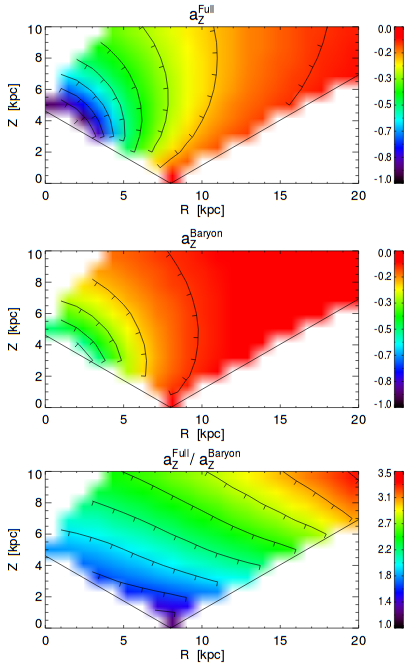
\includegraphics[width=0.8\linewidth]{./pics/loebmanAccelerationCurves.png}
\caption{\tiny Simulated $a_z$ comparison: Total Vs Baryon-contribution}
\end{figure}
\end{column}

\begin{column}{.6\textwidth}
\centering
\small
\begin{itemize}

\item Jean's axisymmetric equations relate $a_z , a_R$ with stellar number density $\nu$, mean azimuthal velocity $\overline{v}_{\phi}$ and velocity dispersions.

\item Dark matter contribution can be estimated from observations (SDSS) and Jean's equations \cite[van der Marel 1991]{vanDerMarel1991}.

\item Their result was an oblate halo with $q_{DM} = 0.47 \pm 0.14$.

\end{itemize}

\end{column}

\end{columns}

\end{frame}
%---------------------------------------------------------------------------------------
\begin{frame}

A more interesting approach: The Sagitarius stream with a triaxial halo \cite[Law \& Majewski 2010]{LawMajewski2010}.

\begin{figure}[c]
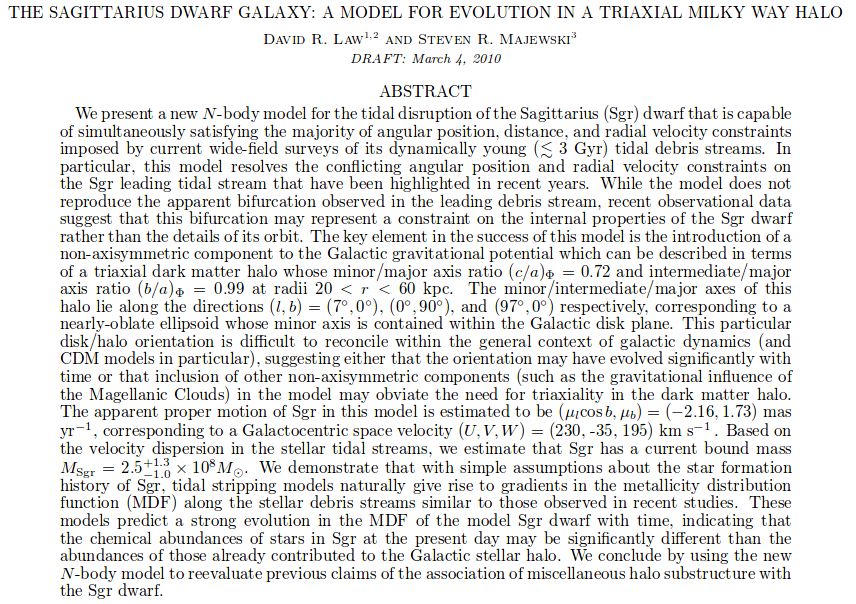
\includegraphics[width=0.8\linewidth]{./pics/LM10.png}
\end{figure}

\end{frame}

%---------------------------------------------------------------------------------------

\begin{frame}

\begin{columns}[c]

\begin{column}{.5\textwidth}
\begin{figure}
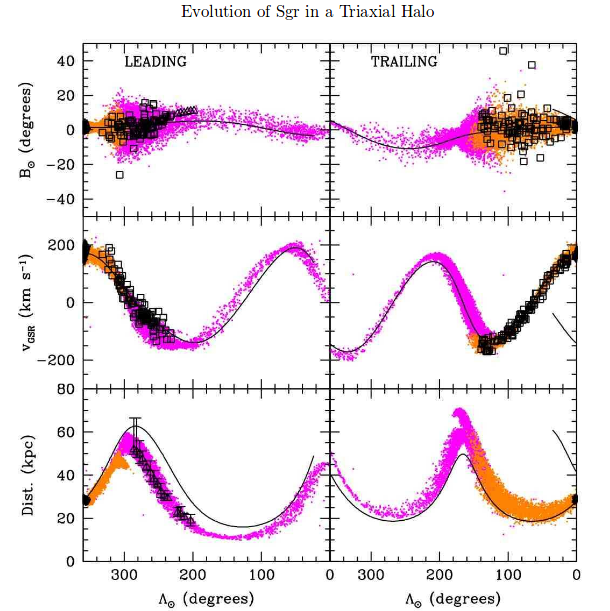
\includegraphics[width=1\linewidth]{./pics/sagStream.png}
\caption{\tiny Simulated Sagitarius stream (color) vs Observed properties of the stream (figures)}
\end{figure}
\end{column}

\begin{column}{.6\textwidth}
\centering
\small
\begin{itemize}

\item Characterization of the sagitarius stream.

\item Variation of parameters: Match simulations with observations.

\item Mismatch between an axisymmetric halo and observations.

\item The best fit parameters are $c/a = 0.72$, $b/a = 0.99$ at $20<r<60 kpc$. 

\item Axis orientation

\end{itemize}

\end{column}

\end{columns}

\end{frame}

%---------------------------------------------------------------------------------------
\begin{frame}
Strong assumptions or simplifications:

\begin{itemize}
\item \textbf{Loebman et al.}: DM halo is perfectly oblate, cylindric Jean's equations.

\item \textbf{Law \& Majewski}: Approximation of stream as CM. Omission of LMC.
\end{itemize}

Observational difficulties:

\begin{itemize}
\item Perpendicular velocities

\item Radial mass distribution
\end{itemize}

\end{frame}

%---------------------------------------------------------------------------------------
\subsection{The utility of Cosmological simulations}

\begin{frame}

Support tool for observation and theory.\\~\\

Evolution of DM and gas in a $\Lambda CDM$ cosmology:

\begin{block}{Self-gravitating collisionless fluid for DM}
\tiny
\begin{align}
\frac{d\rho}{dt} = \frac{\partial \rho}{\partial t} +\vec{v}\cdot\frac{\partial\rho}{\partial \vec{x}}
+\frac{\partial \Phi}{\partial \vec{x}}\cdot\frac{\partial\rho}{\partial \vec{v}}
\end{align}
\end{block}

\begin{block}{Non-viscid thermal fluid for the gas}
\tiny
\begin{align}
&\frac{d\rho}{dt} + \rho \vec{\nabla}\cdot\vec{v} = 0\\
&\frac{d\vec{v}}{dt} = -\frac{\vec{\nabla}P}{\rho} - \vec{\nabla} \Phi \\
&\frac{du}{dt} = -\frac{P}{\rho}\vec{\nabla}\cdot\vec{v} - \frac{\vec{\Lambda(u,\rho)}}{\rho}\\
& P = (\gamma -1 )\rho u
\end{align}
\end{block}
\end{frame}

%---------------------------------------------------------------------------------------
%---------------------------------------------------------------------------------------
\begin{frame}

\begin{columns}[c]

\begin{column}{.5\textwidth}
\begin{figure}
\includegraphics[width=1\linewidth]{./pics/Auriga.png}
\caption{\tiny Auriga simulations. http://auriga.h-its.org}
\end{figure}
\end{column}

\begin{column}{.6\textwidth}
\centering
\footnotesize
\begin{itemize}

\item Evolution: SPH MMH.
\item Energetic feedback.
\item We focus on AURIGA \cite{auriga} simulations made with AREPO \cite{arepo}.
\item Various degrees of realism.
\item Magnetic fields.

\end{itemize}

\end{column}

\end{columns}

\end{frame}

%---------------------------------------------------------------------------------------
\subsection{Simulations and observations}
\begin{frame}

A study of the shape in terms of the radius and history.

\begin{figure}[c]
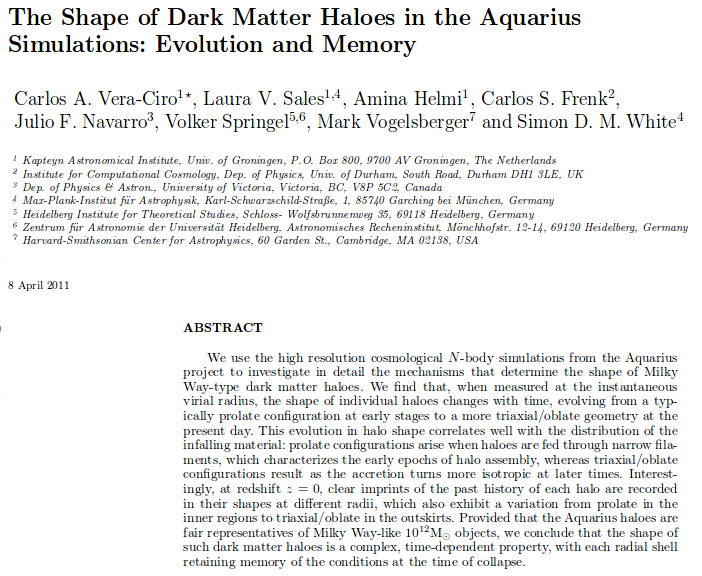
\includegraphics[width=0.8\linewidth]{./pics/veraCiroAquarius.png}
\end{figure}

\end{frame}

%---------------------------------------------------------------------------------------

\begin{frame}

\begin{columns}[c]

\begin{column}{.4\textwidth}
\begin{figure}
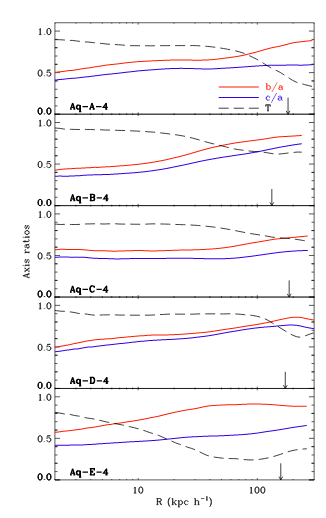
\includegraphics[width=0.8\linewidth]{./pics/shapeRadius.png}
\caption{\tiny Dependence of shape on radius}
\end{figure}
\end{column}

\begin{column}{.7\textwidth}
\centering
\begin{figure}
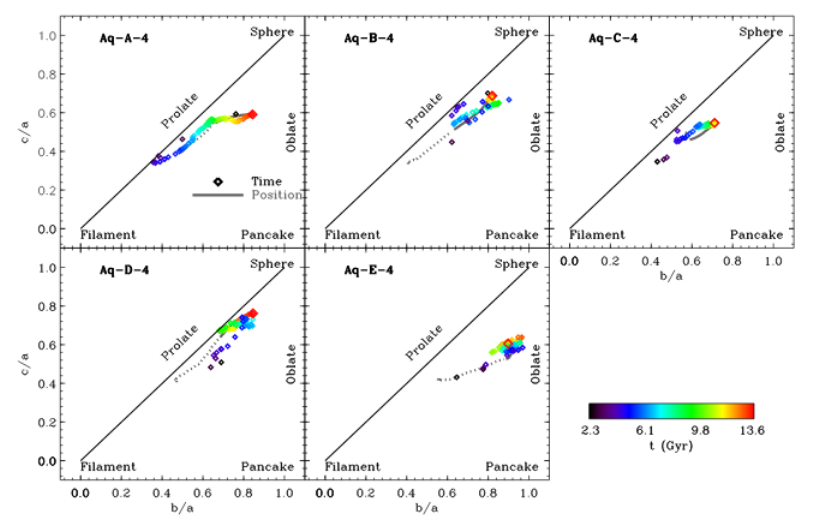
\includegraphics[width=1\linewidth]{./pics/shapeHistory.png}
\caption{\tiny Dependence of shape on history}
\end{figure}

\end{column}

\end{columns}

\end{frame}

%---------------------------------------------------------------------------------------
\begin{frame}

Aquarius simulations \cite{aquarius}.\\~\\

Shape in terms of radius? How to measure it? \\~\\

Their main results are: 

\begin{itemize}
\item Dependence on the radius.

\item Correlation of historical shape and present shape.

\item Halos evolve towards prolate shapes.

\end{itemize}

\end{frame}


%---------------------------------------------------------------------------------------
\begin{frame}

Improvement on observational constraints:

\begin{figure}[c]
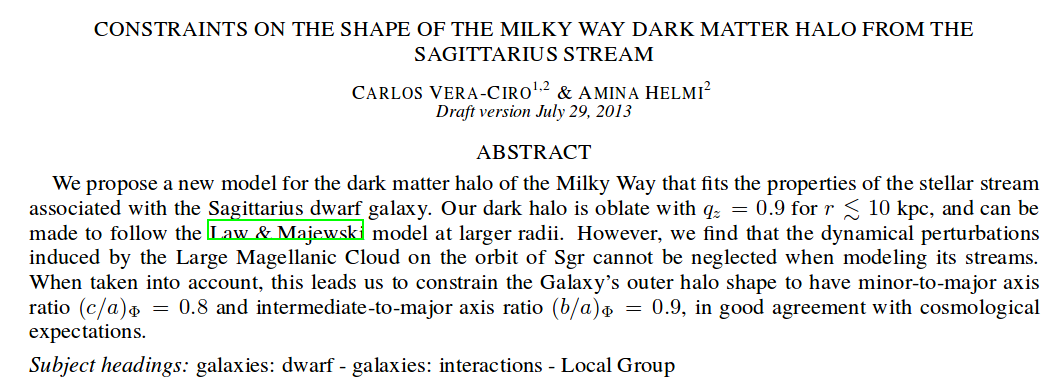
\includegraphics[width=1\linewidth]{./pics/veraCiroSagitarius.png}
\end{figure}

\end{frame}

%---------------------------------------------------------------------------------------

\begin{frame}

Iprovement of Law \& Majewski 2010 study with relaxed asumptions.\\~\\

The DM halo assumptions:

\begin{itemize}
\item Axisymmetric at inner parts, \textbf{coherent with the MW disk}.

\item Triaxial on the outer-skirts.

\item Smooth transition.

\end{itemize}

They used variation of parameters yield:

\begin{itemize}
\item $qz = 0.9$ at $r \approx 10kpc$

\item $b/a = 0.9, c/a = 0.8$ at $r>>30kpc$

\end{itemize}

\end{frame}

%---------------------------------------------------------------------------------------
\section{Our study}
\subsection{Objectives}
\begin{frame}

\begin{itemize}
\item Study the shape of the DM halo in terms of the radius in the AURIGA simulations.

\item Study the correlation of the radial and historical profiles.

\item \textbf{\textit{Analyze the relation or the effect of baryons on the DM halo shape.}}

\end{itemize}

\end{frame}

%---------------------------------------------------------------------------------------
\subsection{How do we calculate DM shapes in terms of radius? (simulations)}
\begin{frame}
\footnotesize
We follow Vera-Ciro et al. 2011 (Allgood et al. 2006) to calculate shapes.\\~\\

Shapes are determined by the semiaxes $a,b,c$ of the ellipsoid associated to the halo.\\~\\

First we choose a radius $R$. We calculate the reduced inertia tensor for all particles within the defined sphere:

\begin{equation}
I_{ij} = \sum_k \frac{x_k^{(i)}x_k^{(j)}}{d^2_k}
\end{equation}

The eigenvalues of this tensor are said semiaxes along the corresponding eigenvectors.\\~\\

But this is not sufficient: Calculate ellipse from spherical selection of particles.

\end{frame}


%---------------------------------------------------------------------------------------
\begin{frame}
\small

The solution is to rescale positions for the current ellipse to become a sphere and recalculate:\\~\\

Once obtained the first semiaxes, we rescale:

\begin{align}
(x,y,z) &\rightarrow (x,y/q,z/s) \\
q &=  b/a\\
s &= c/a,
\end{align}

This rescaling is used to redefine the contour \textit{sphere} and to calculate the \textit{distance} in the inertia tensor.\\~\\

The semiaxes are recalculated the rescaling is performed iteratively until we achieve convergence: changes in semiaxes are less than $10^{-6}$


\end{frame}

%---------------------------------------------------------------------------------------
\subsection{Convergence analysis}
\begin{frame}
\begin{figure}[!ht]
  \centering
  \subfloat[halo 24 MHD]{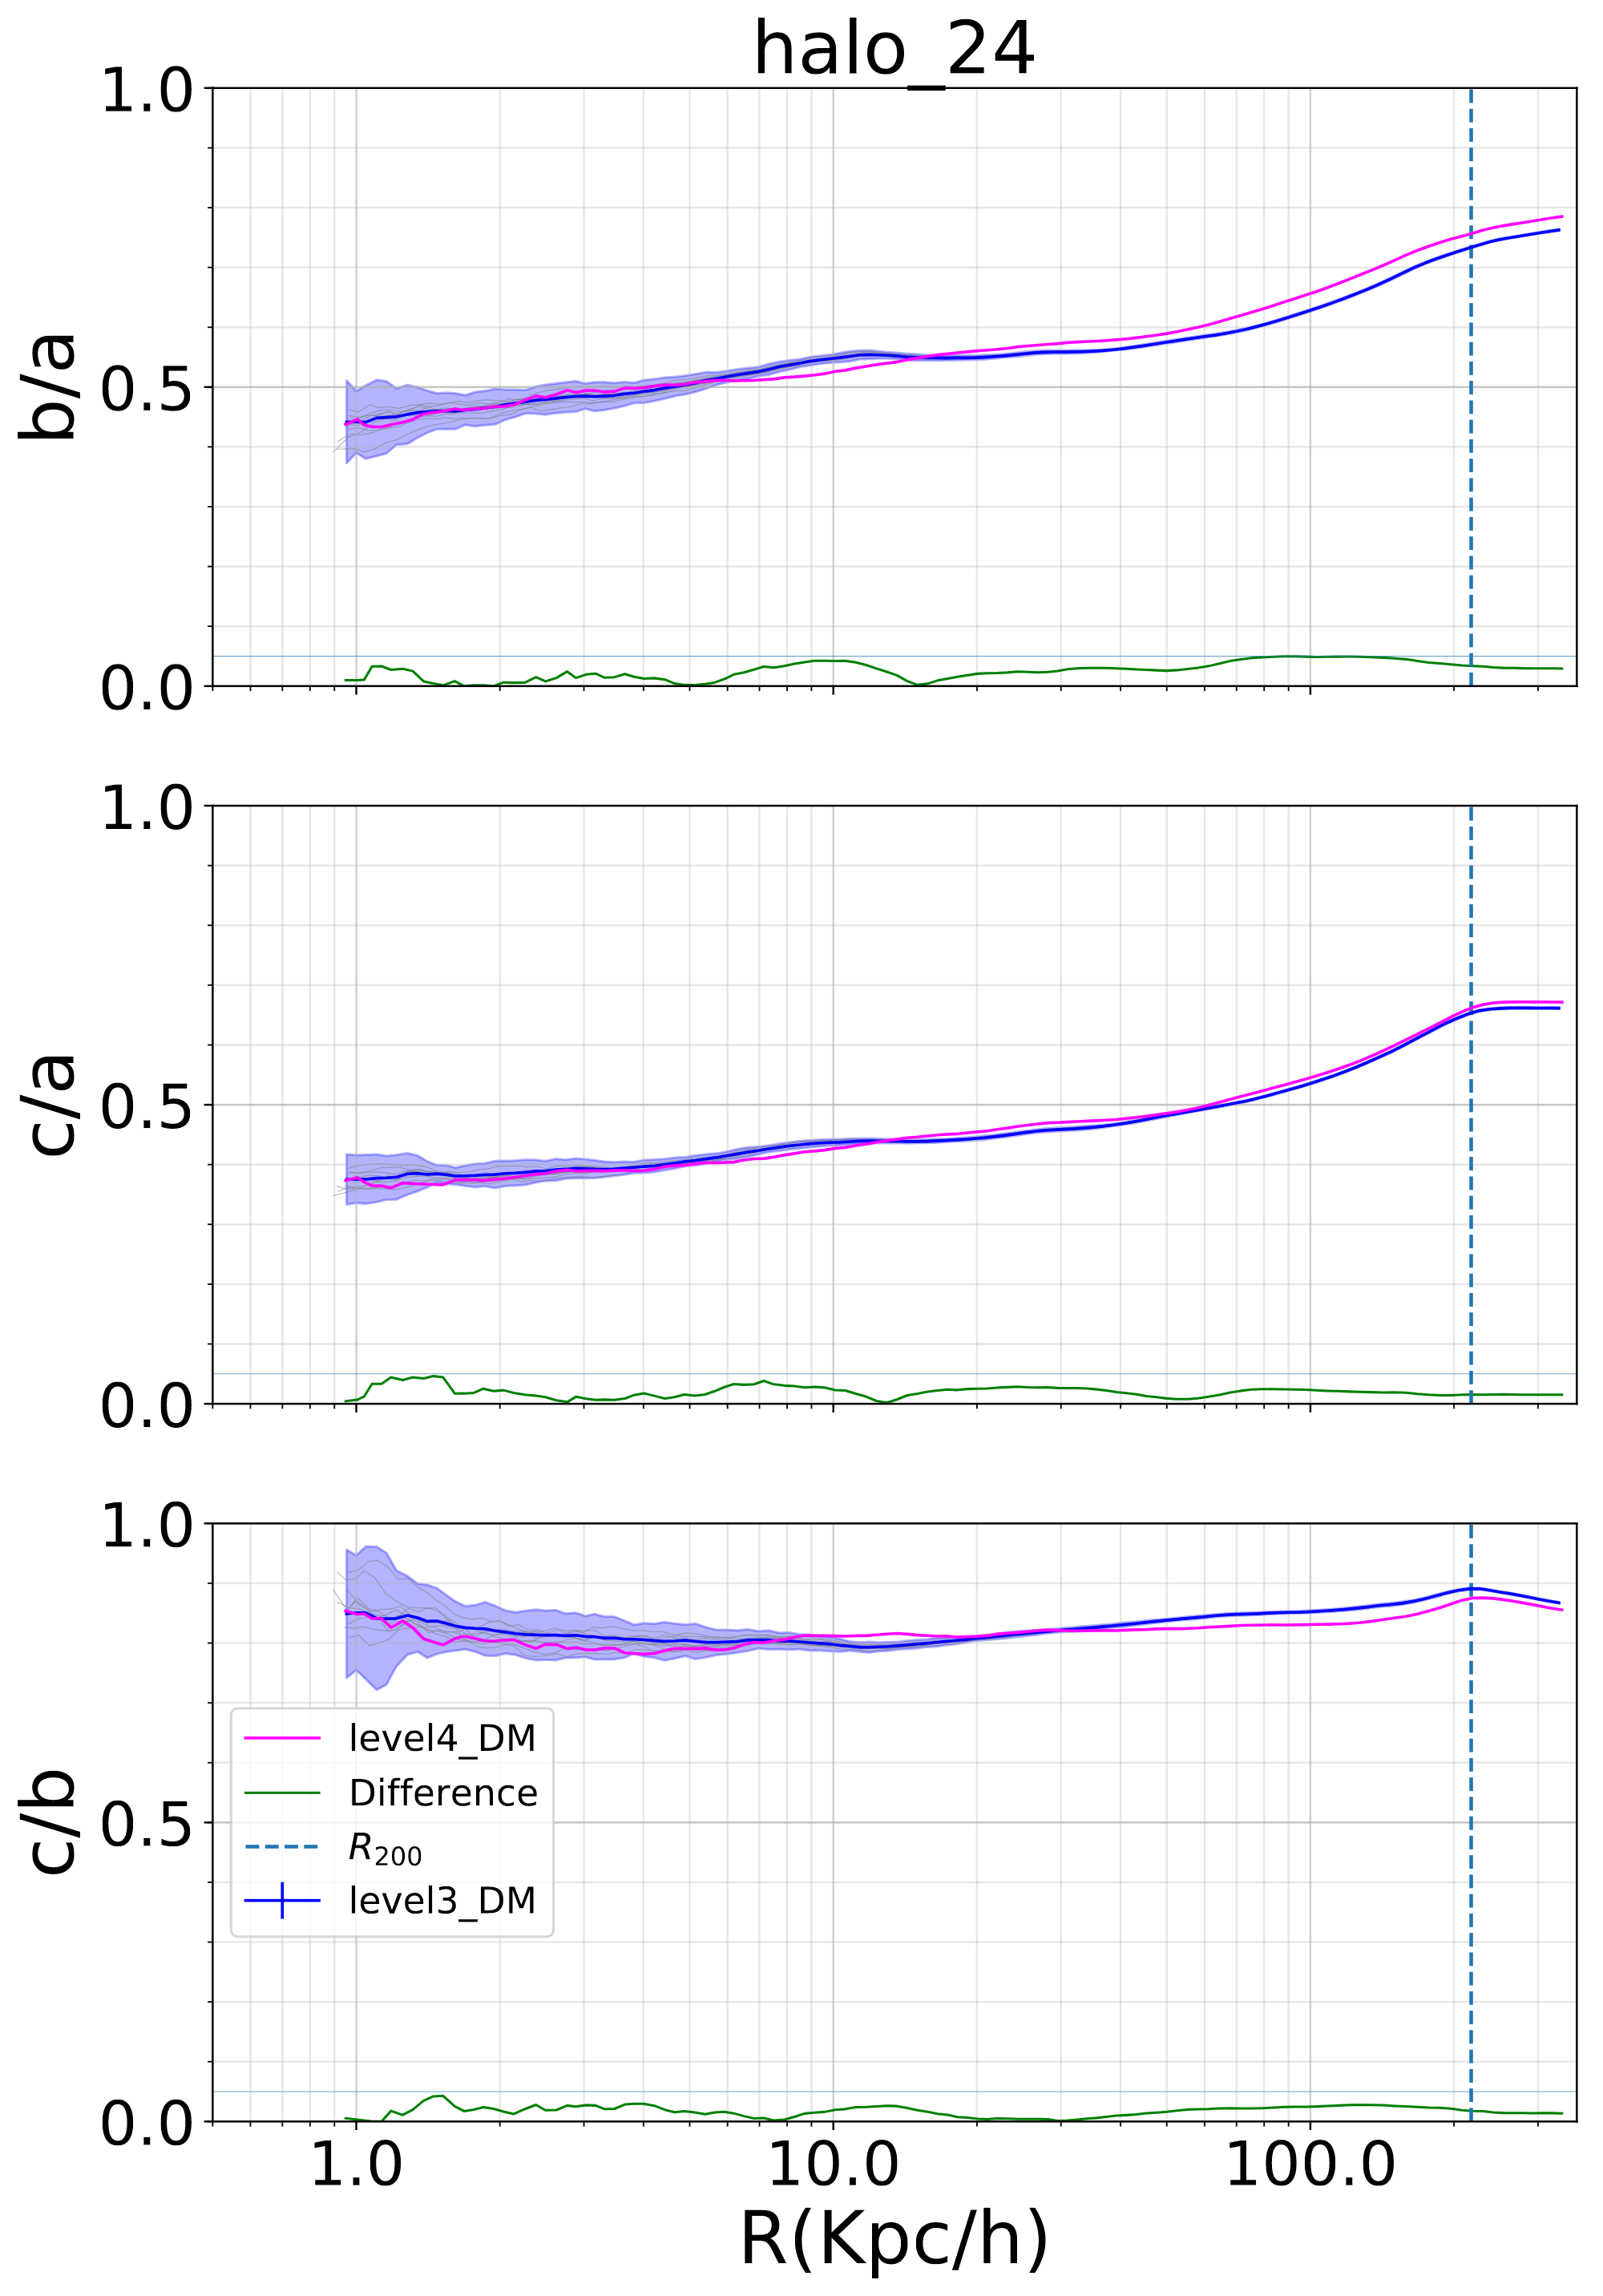
\includegraphics[width=0.45\columnwidth]{../Document/pics/Convergence/rand_conv_halo24_DM.png}}
  \hfill
  \subfloat[halo 24 DM]{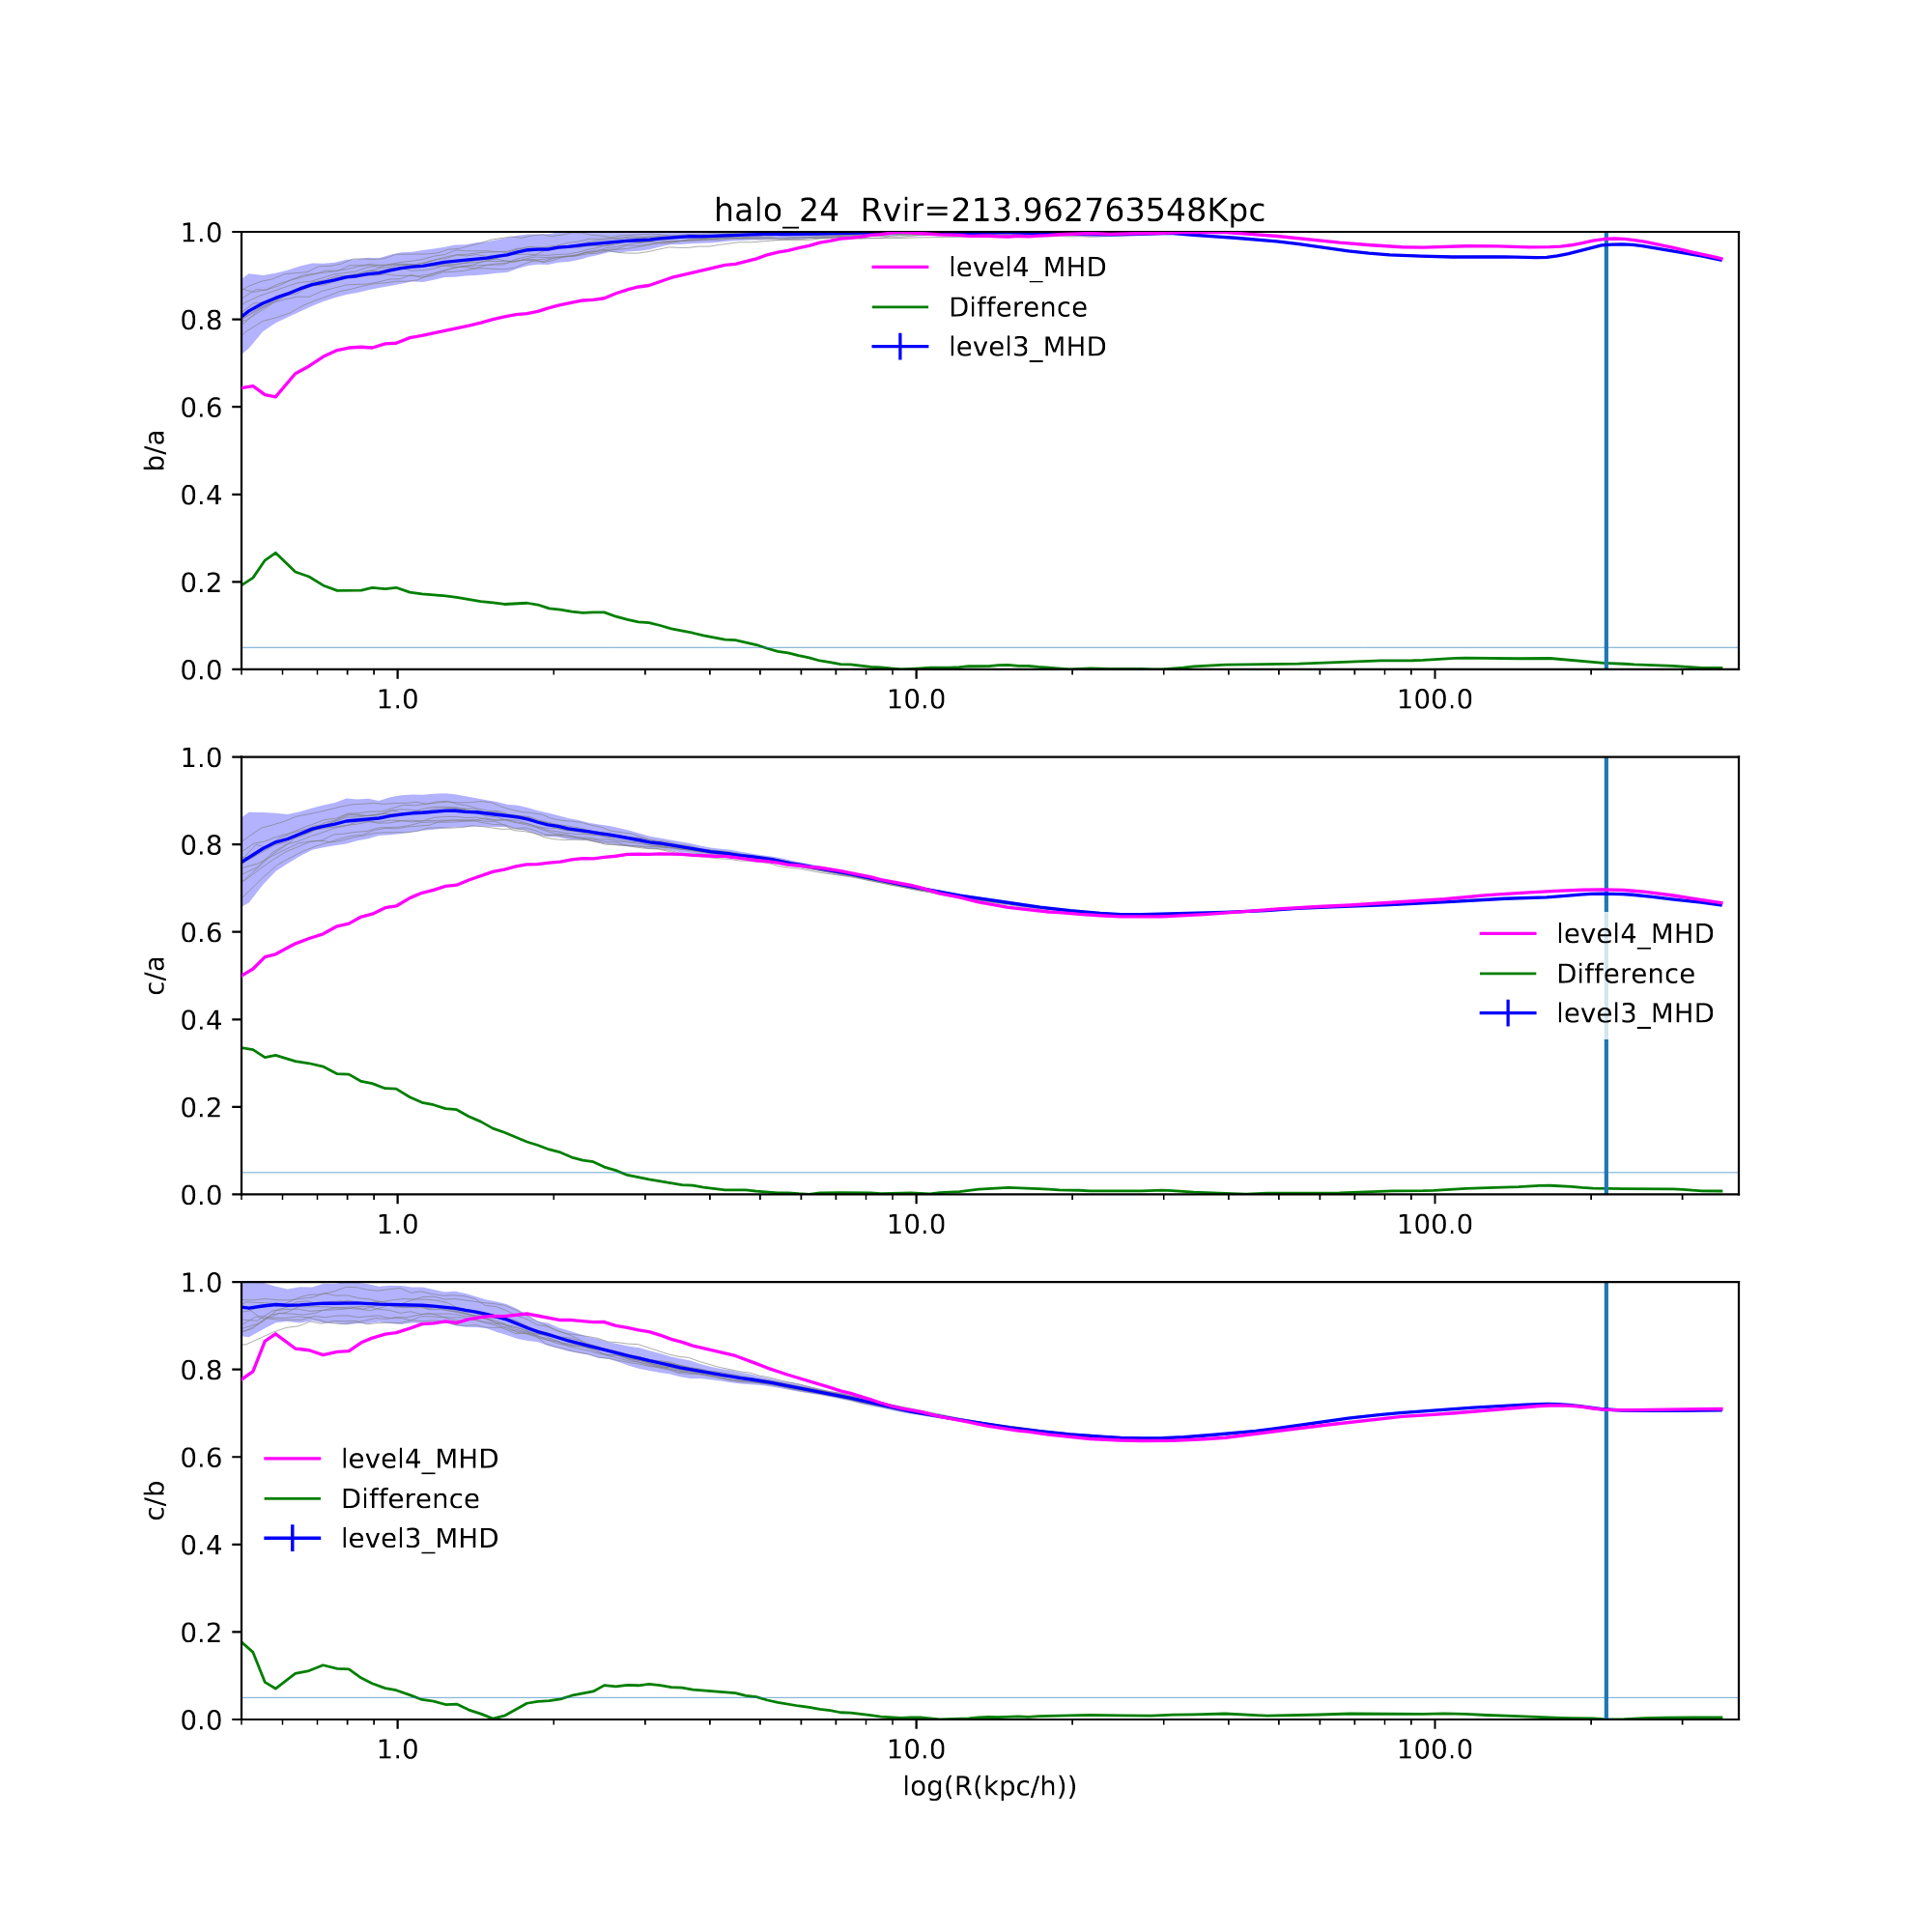
\includegraphics[width=0.45\columnwidth]{../Document/pics/Convergence/rand_conv_halo24_MHD.png}}
  %\caption{The few-particle effect on the axial ratios convergence for halo 24 (DM \& MHD). Here level4 curves (magenta) are compared to  the 3$\sigma$ range (clear blue) of the random-sampled curves from level3 (solid blue). We deduce from the fractional difference (green) that discrepancies at $r>>1$Kpc cannot be explained solely with the few-particle bias. }
  \label{fig:convergence}  
\end{figure}
\end{frame}

%---------------------------------------------------------------------------------------
\begin{frame}
\begin{figure}
\centering
\subfloat{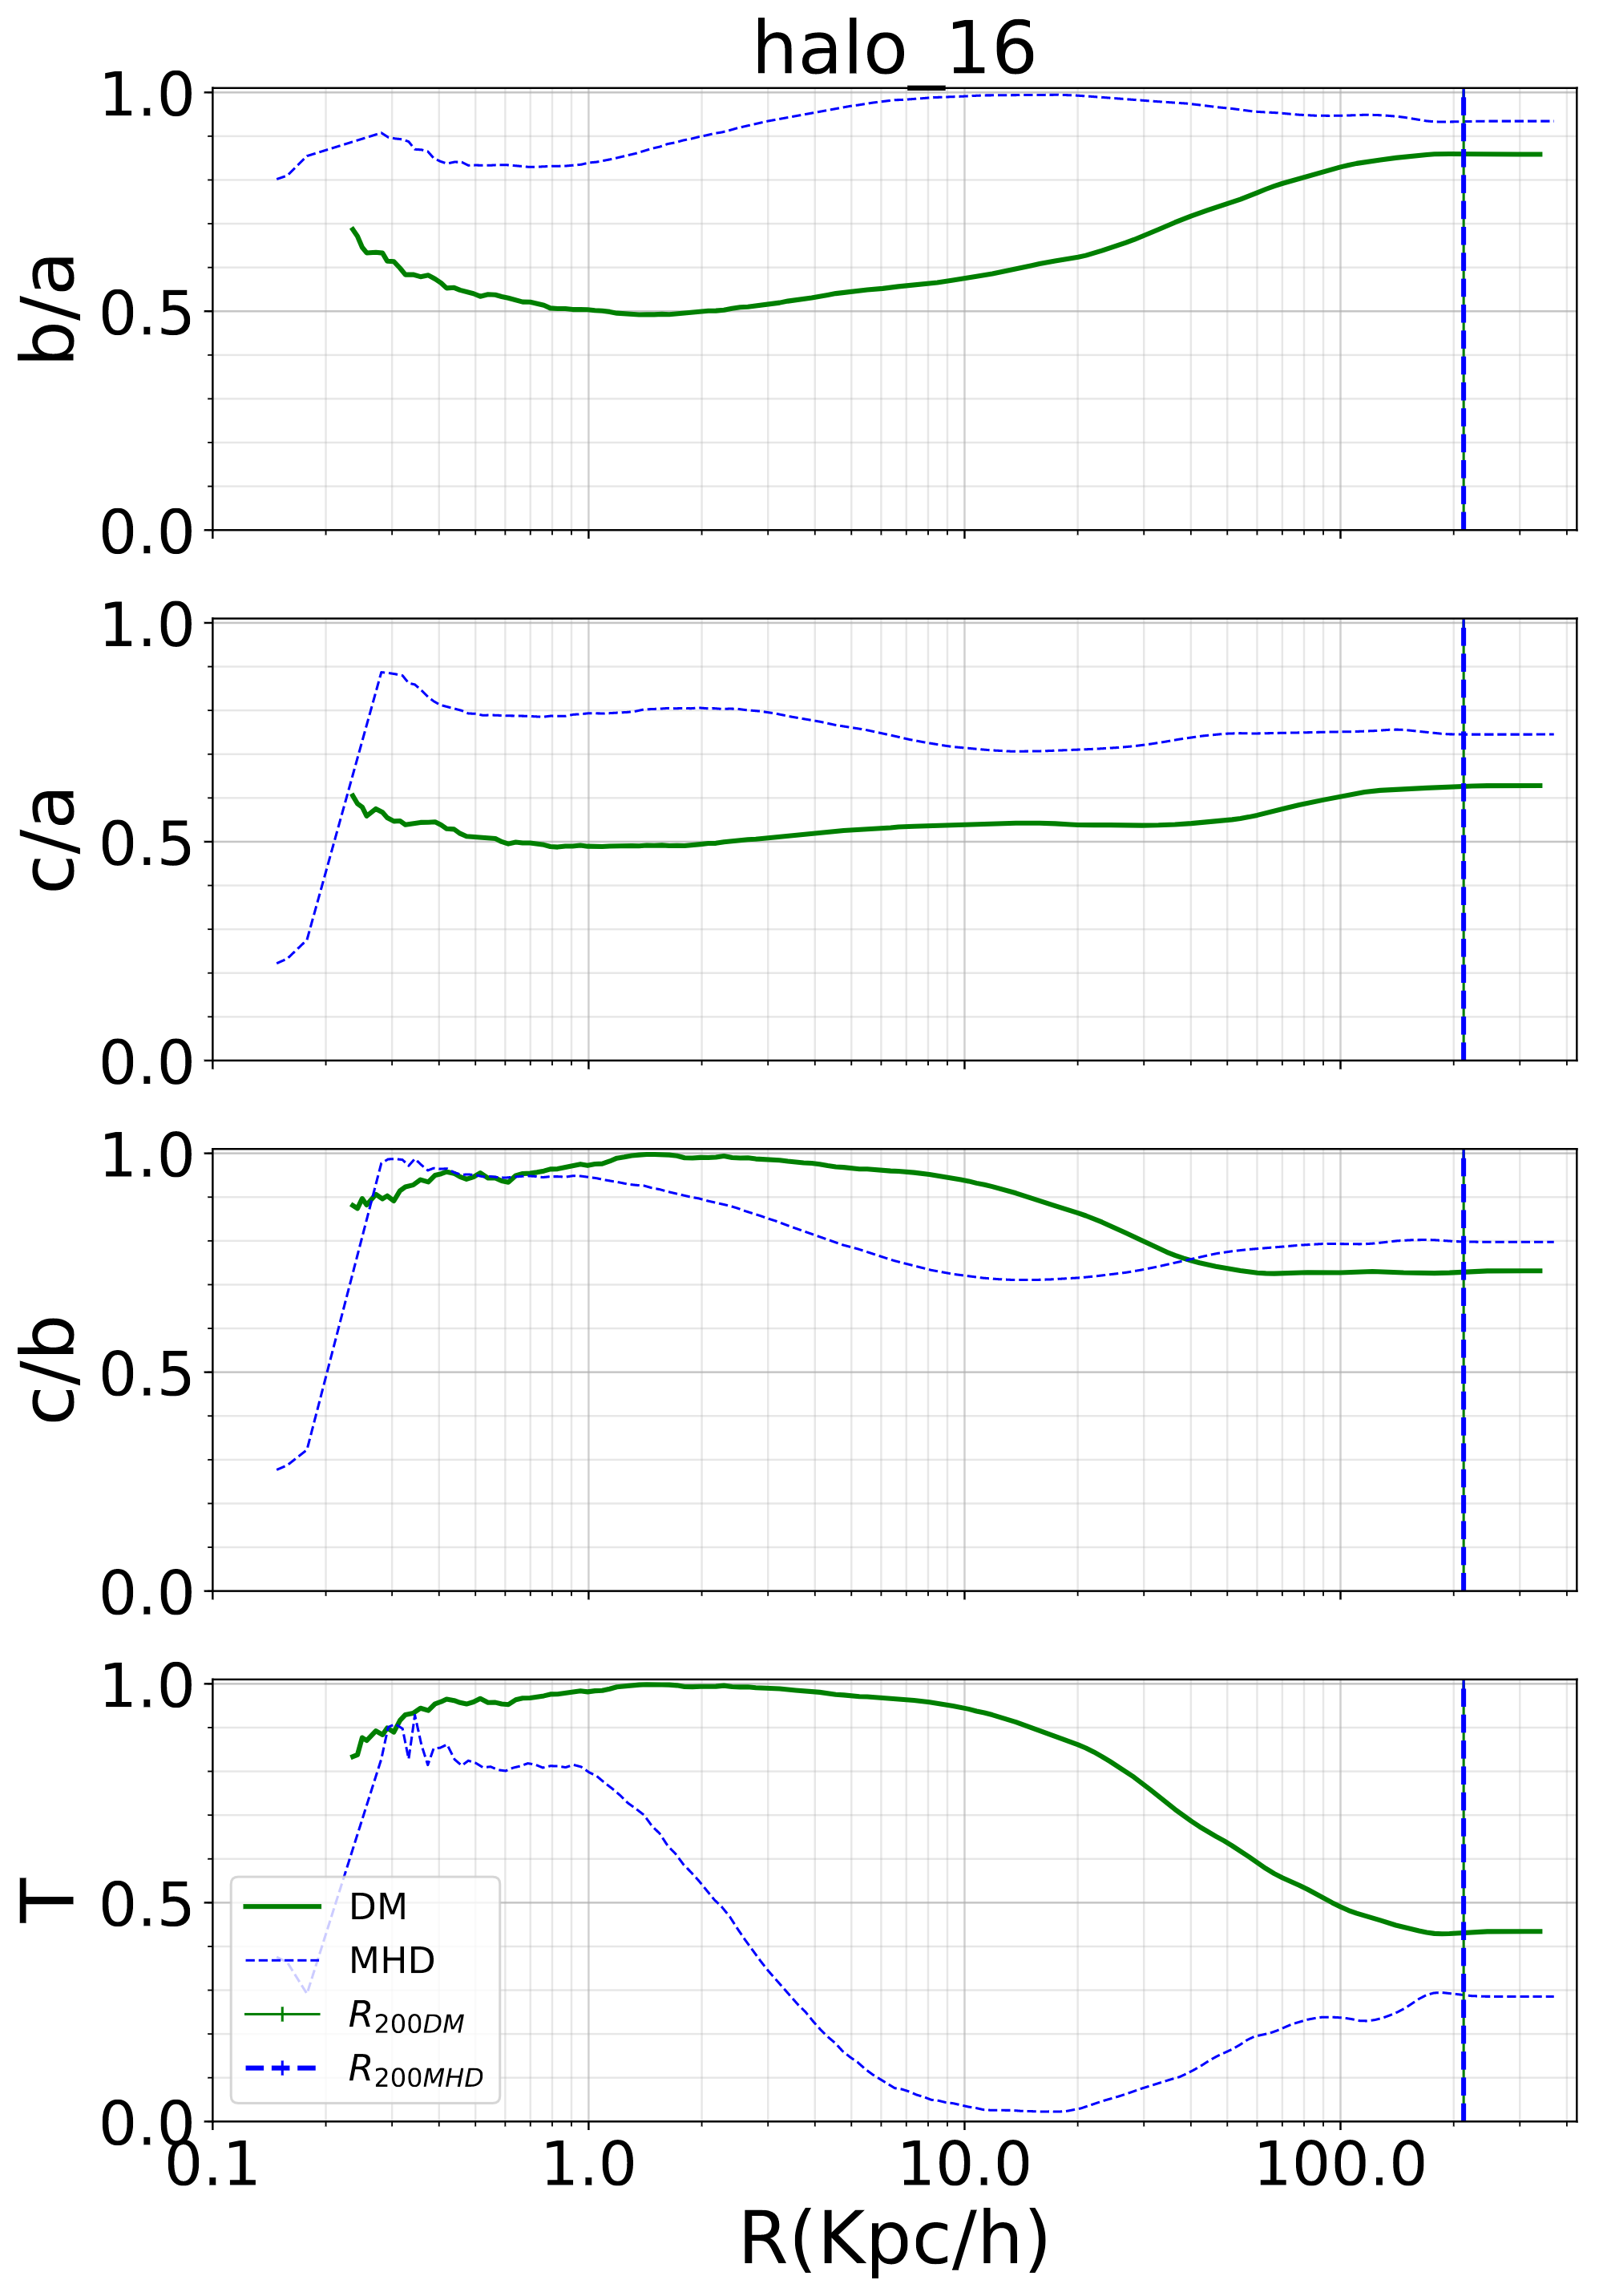
\includegraphics[width=0.45\columnwidth]{../Document/pics/halo16.png}}
  \hfill
\subfloat{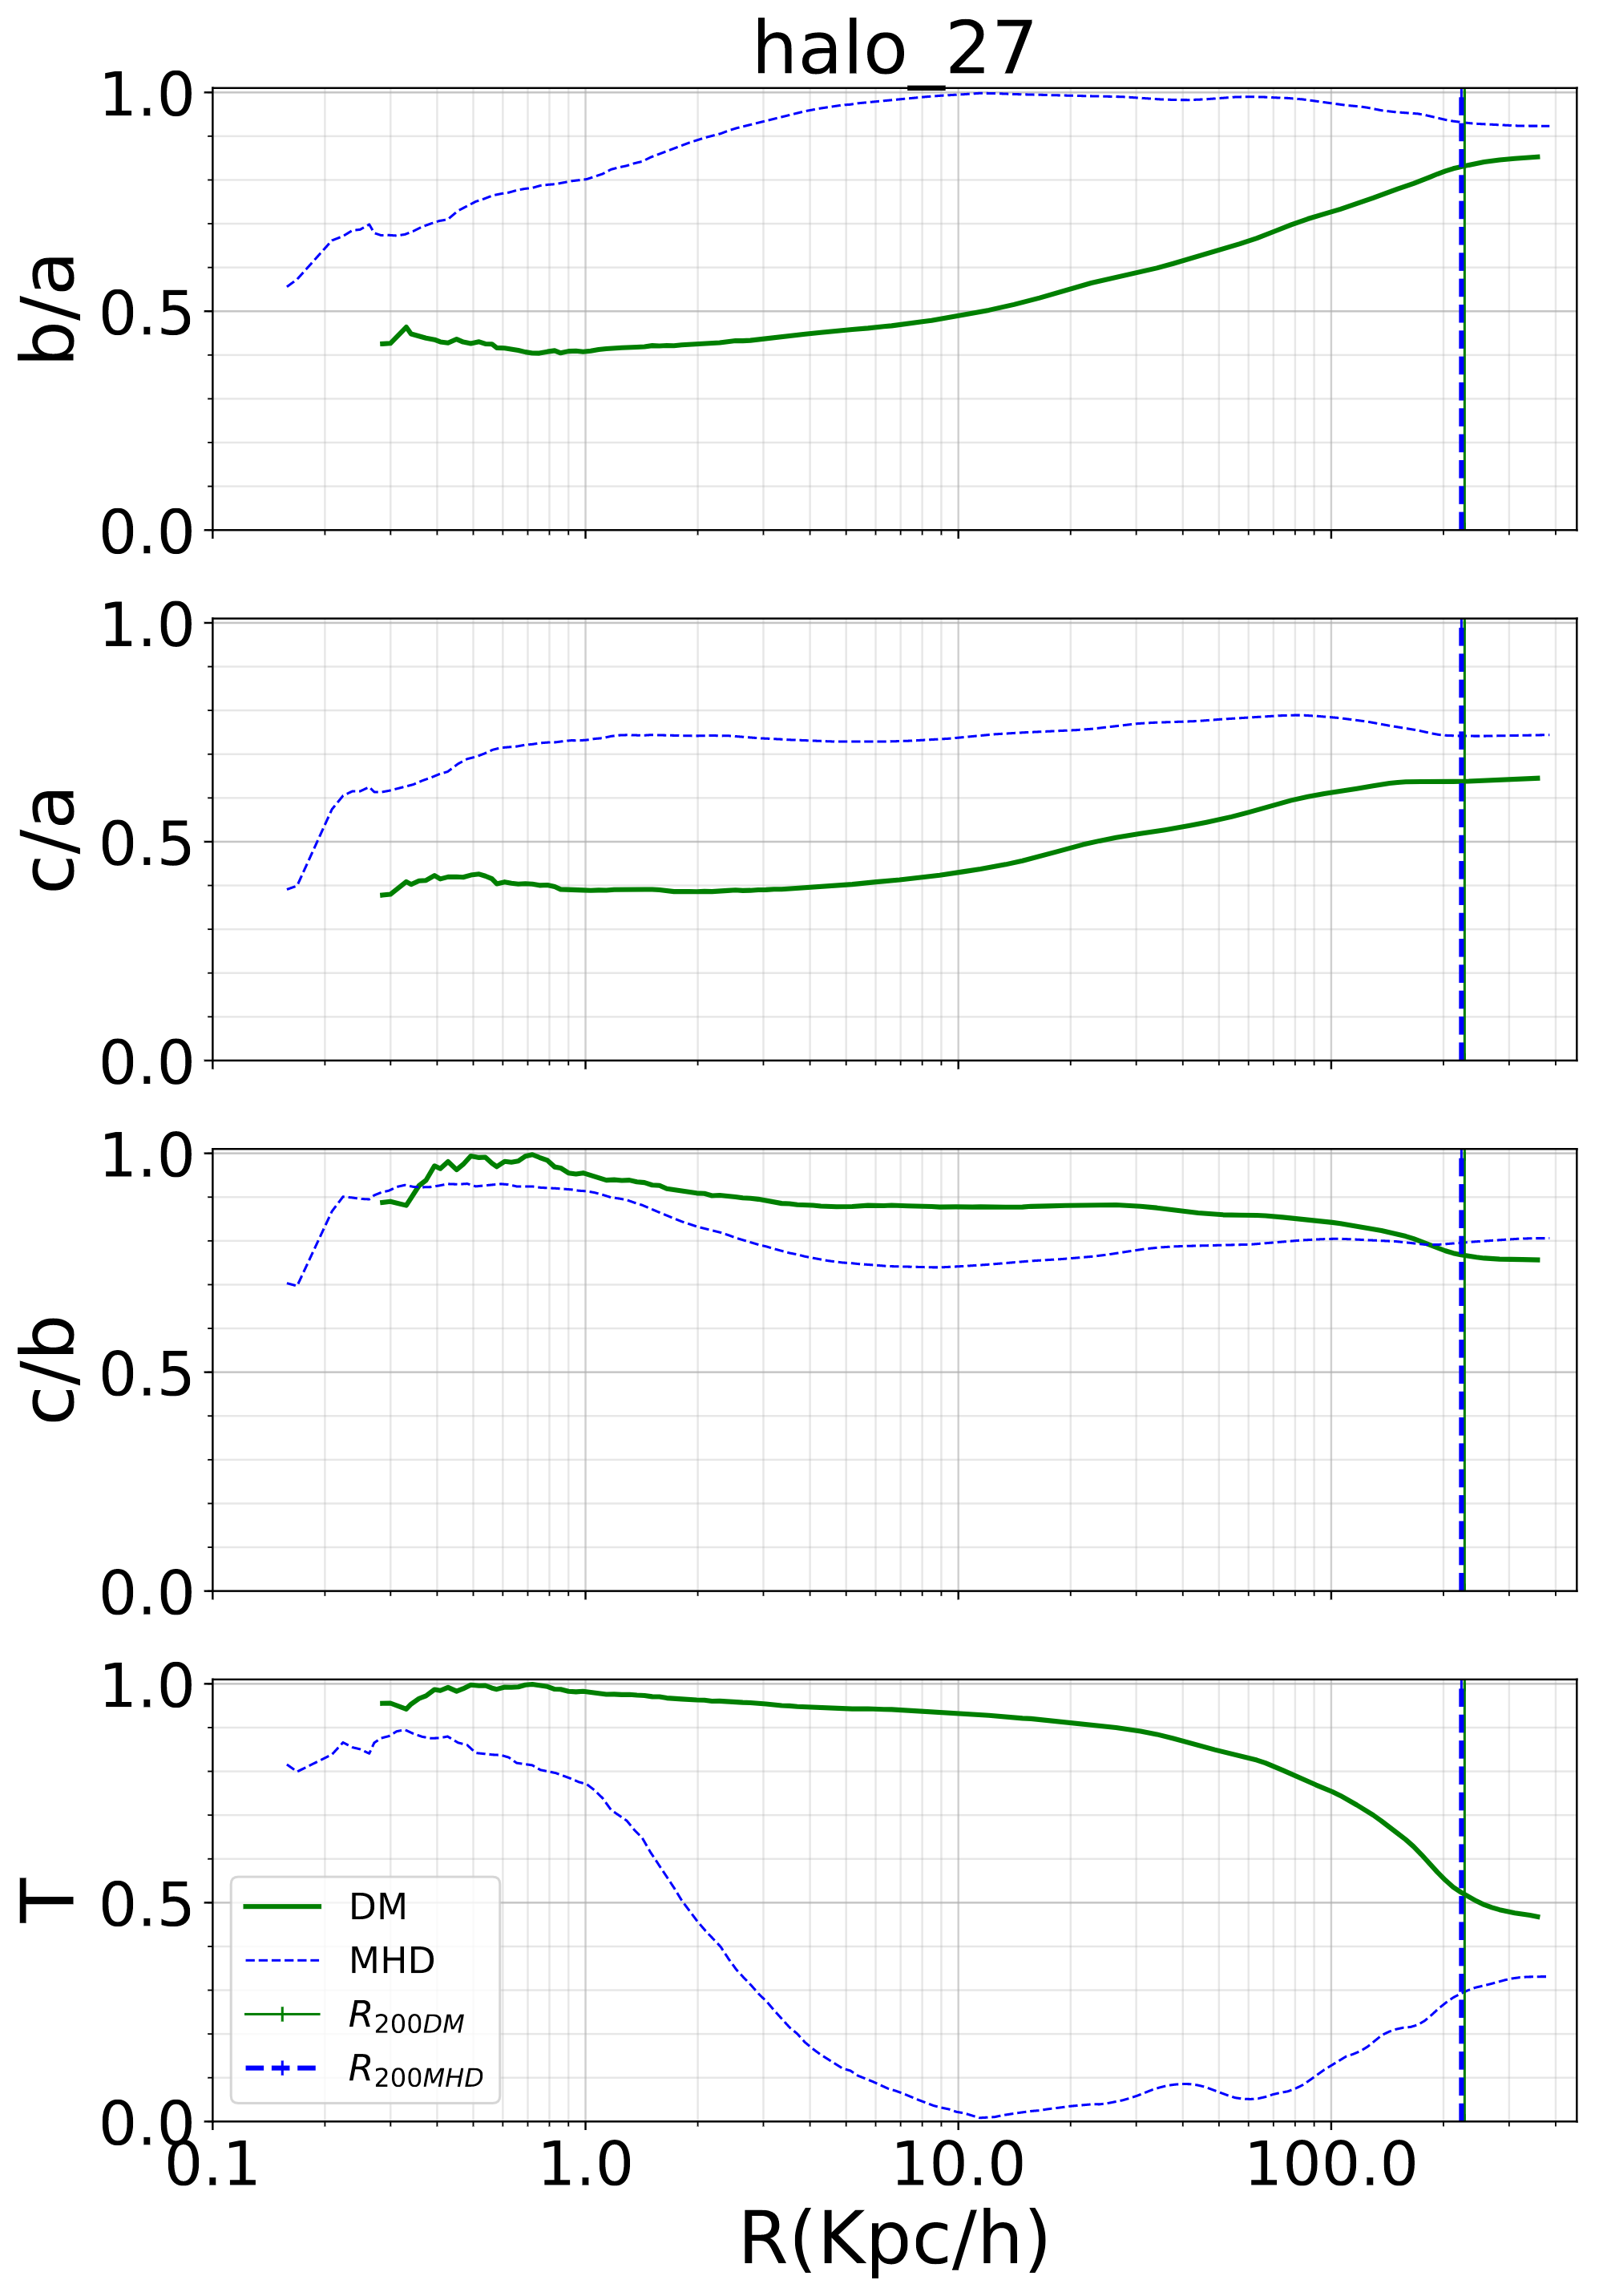
\includegraphics[width=0.45\columnwidth]{../Document/pics/halo27.png}}

%\caption{Radial profile for axial ratios and the triaxiality parameter $T=\frac{1-b/a}{1-c/a}$ from halo 27 and halo 16. These halos have a clear radial tendence towards sphericity (for smaller radii until $\approx 3$Kpc), which can be confirmed with the triaxiality parameter. }
\label{fig:DM_MHD}
\end{figure} 

\end{frame}

%---------------------------------------------------------------------------------------
\subsection{Radial dependence of shape}
\begin{frame}[plain]

\begin{figure}[!ht]
  \centering
  \subfloat[\tiny halo 27 DM shape (small radius)]{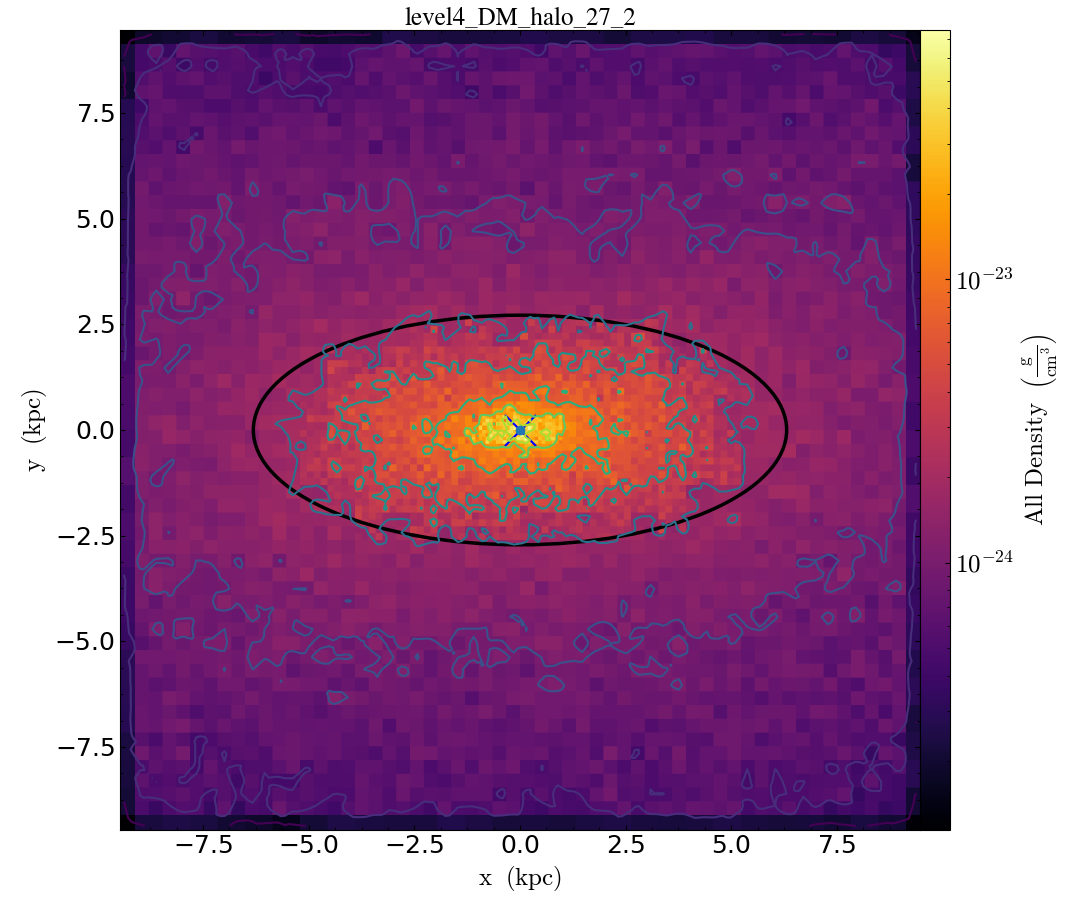
\includegraphics[width=0.4\columnwidth]{../Document/pics/MHD_Vs_DM/level4_DM_halo_27_inner.png}}
  \hfill
  \subfloat[\tiny halo 27 DM shape (big radius)]{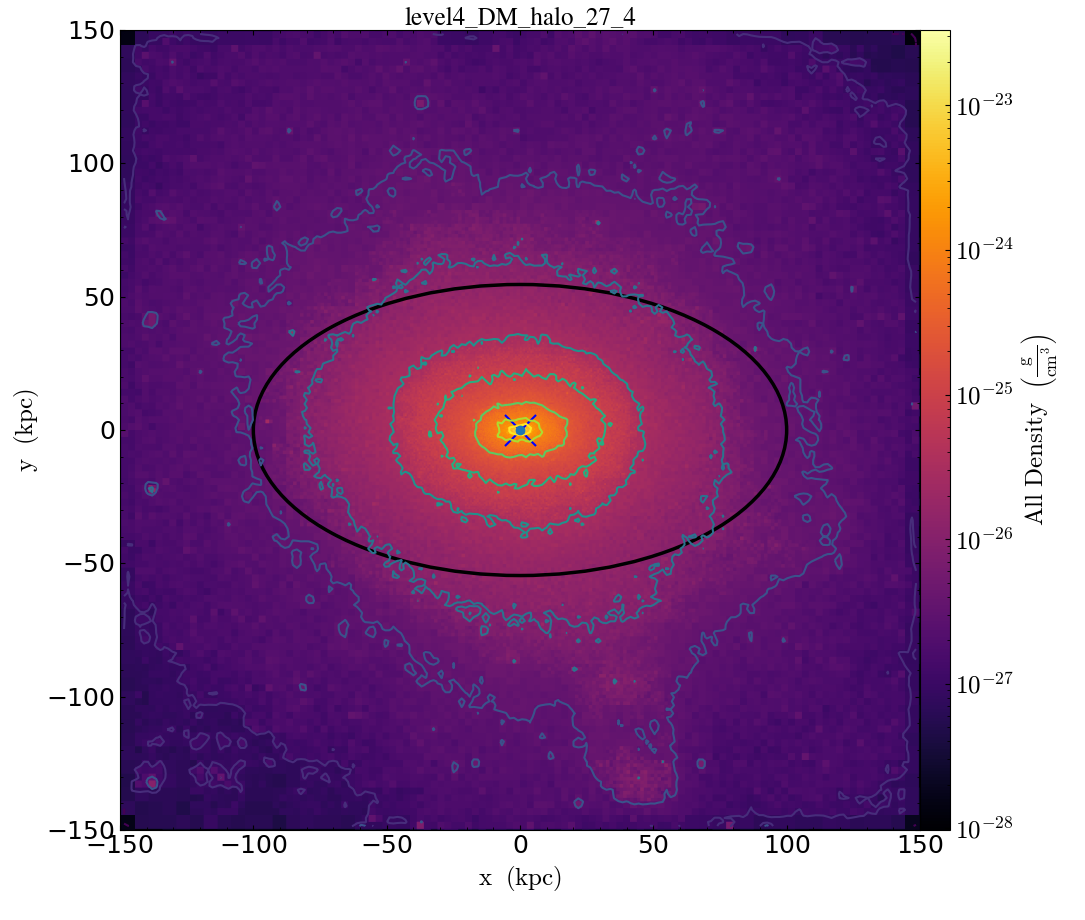
\includegraphics[width=0.4\columnwidth]{../Document/pics/MHD_Vs_DM/level4_DM_halo_27_outter.png}}
  \hfill
  \subfloat[\tiny halo 27 MHD shape (small radius)]{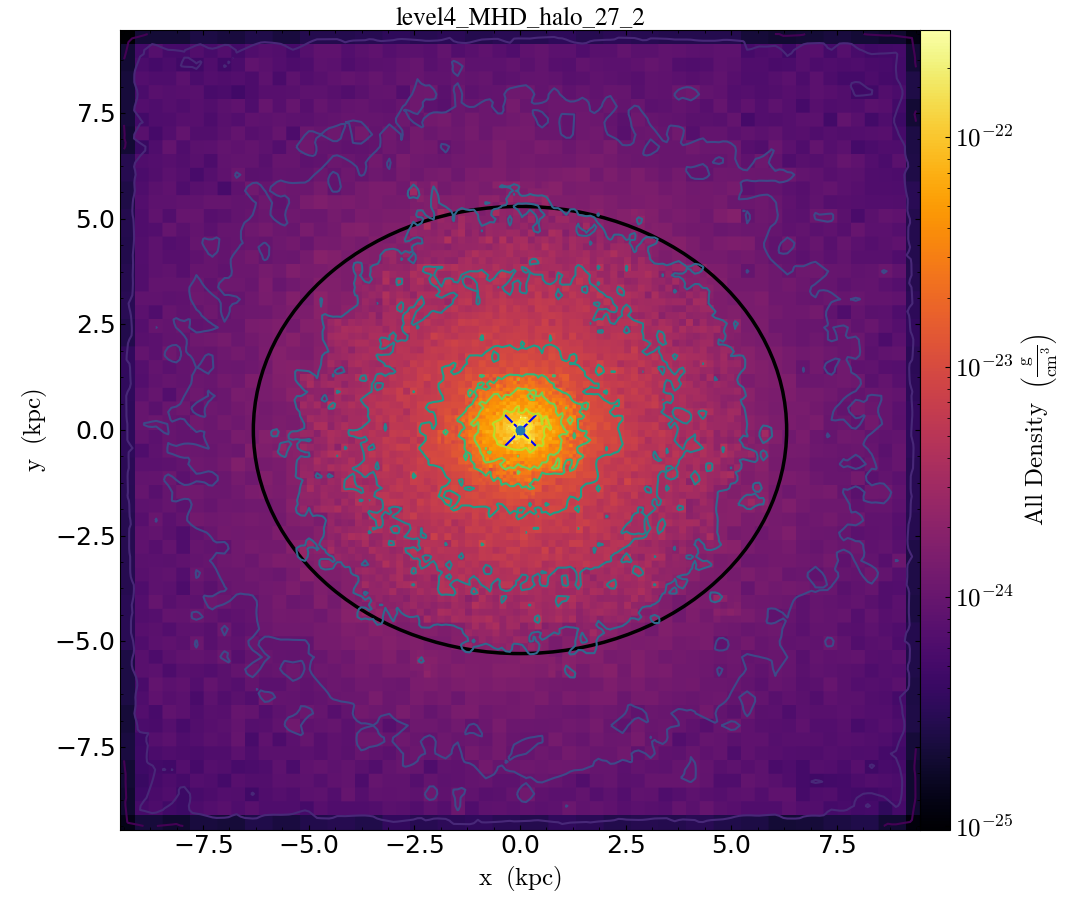
\includegraphics[width=0.4\columnwidth]{../Document/pics/MHD_Vs_DM/level4_MHD_halo_27_inner.png}}
  \hfill
  \subfloat[\tiny halo 27 MHD shape (big radius)]{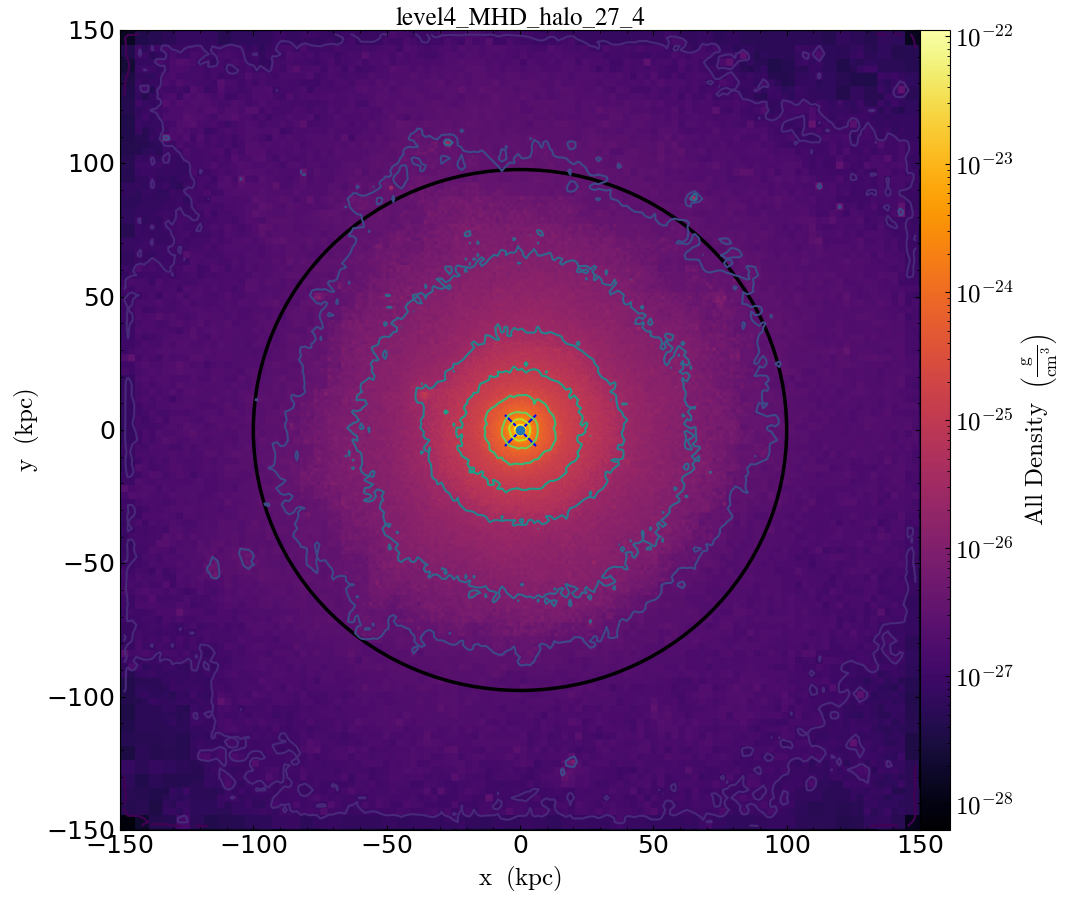
\includegraphics[width=0.4\columnwidth]{../Document/pics/MHD_Vs_DM/level4_MHD_halo_27_outter.png}}
 % \caption{DM density for inner (left) and outer (right) parts of the halo 27. We present both versions: DM (up) \& MHD (down). The horizontal and vertical axes are aligned to the major and medium semi-axes respectively. Here, it is evident that this halo is more spherical at bigger radii and more triaxial at the central parts. }
\normalsize
  \label{fig:slices}
\end{figure}


\end{frame}

%---------------------------------------------------------------------------------------

\begin{frame}[plain]

\begin{figure}[!ht]
  \centering
  \subfloat[\tiny Level4 MHD Vs DM at inner regions]{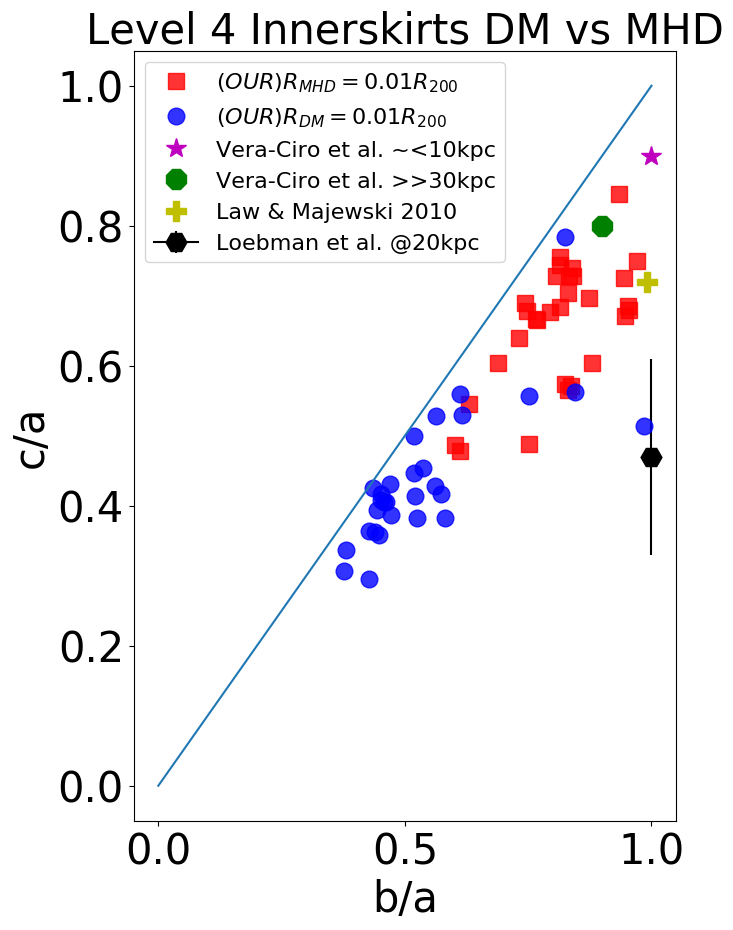
\includegraphics[width=0.5\columnwidth]{../Document/pics/Triaxial_Plane/Triaxiality_Inner_lvl4.png}}
  \hfill
  \subfloat[\tiny Level4 MHD Vs DM at outer regions]{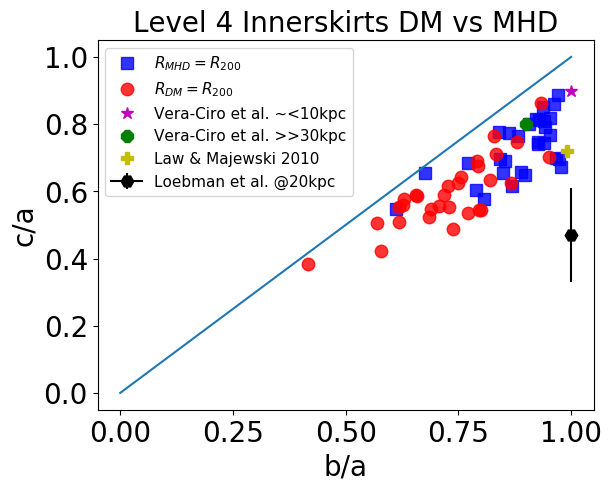
\includegraphics[width=0.5\columnwidth]{../Document/pics/Triaxial_Plane/Triaxiality_Outter_lvl4.png}}
  \hfill
  %\caption{Axial ratios as shown on $c/a$ Vs $b/a$. Each dot represents a halo shape at some radius. Some observational constraints are plotted alongside our results. Here, dots are clustered, proving the general tendence of halos to get rounder on the outer parts. }
  \label{fig:Triaxiality_Inner_Outer}
\end{figure}
\normalsize

\end{frame}

%---------------------------------------------------------------------------------------
\subsection{The effect of gas}
\begin{frame}
\begin{figure}[!ht]
  \centering
  \subfloat[\tiny Level4 DM inner Vs outer regions]{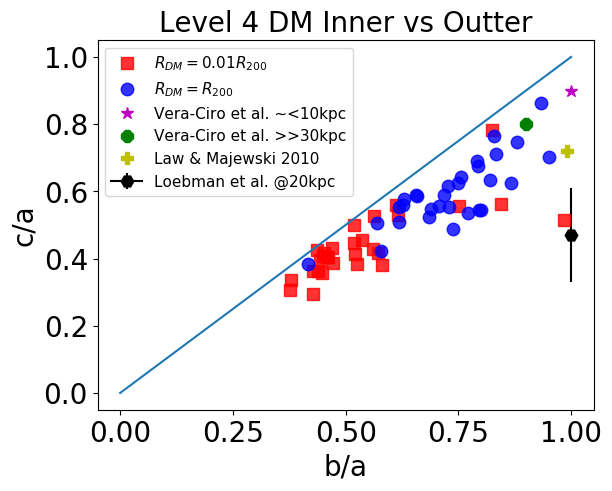
\includegraphics[width=0.5\columnwidth]{../Document/pics/Triaxial_Plane/Triaxiality_DM_lvl4.png}}
  \hfill
  \subfloat[\tiny Level4 MHD inner Vs outer regions]{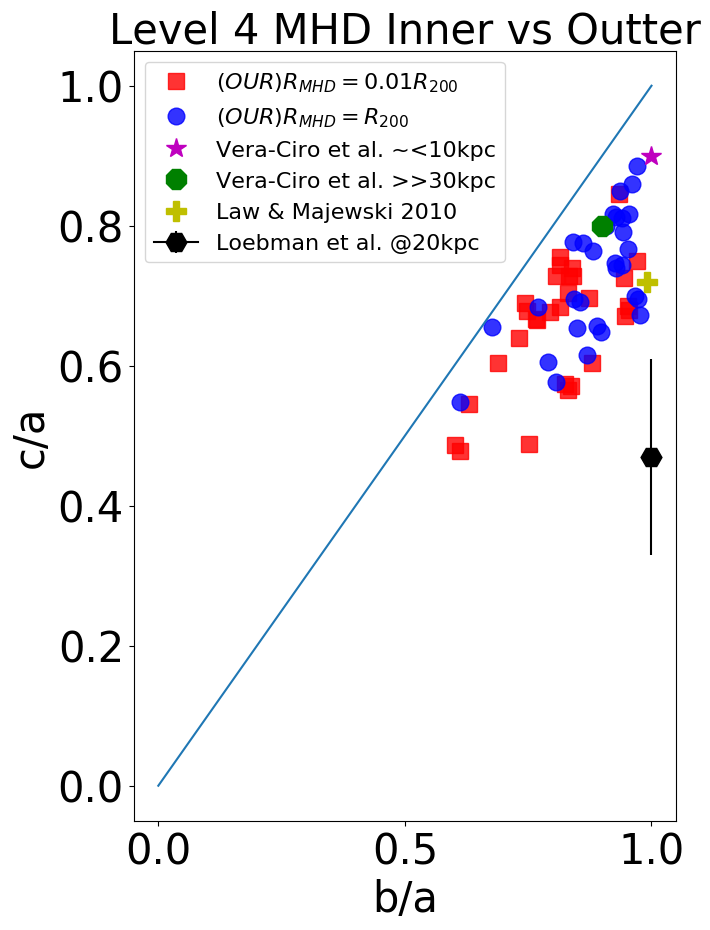
\includegraphics[width=0.5\columnwidth]{../Document/pics/Triaxial_Plane/Triaxiality_MHD_lvl4.png}}
  \hfill
  %\caption{General tendency on the triaxial plane $c/a$ Vs $b/a$. Some observational constraints are plotted alongside our results}
  \label{fig:Triaxiality_DM_MHD}
\end{figure}
\normalsize


\end{frame}

%---------------------------------------------------------------------------------------

%---------------------------------------------------------------------------------------
\subsection{Historical and radial correlations}
\begin{frame}

\begin{figure}[!ht]
  \centering
  \subfloat[\tiny halo 16 DM]{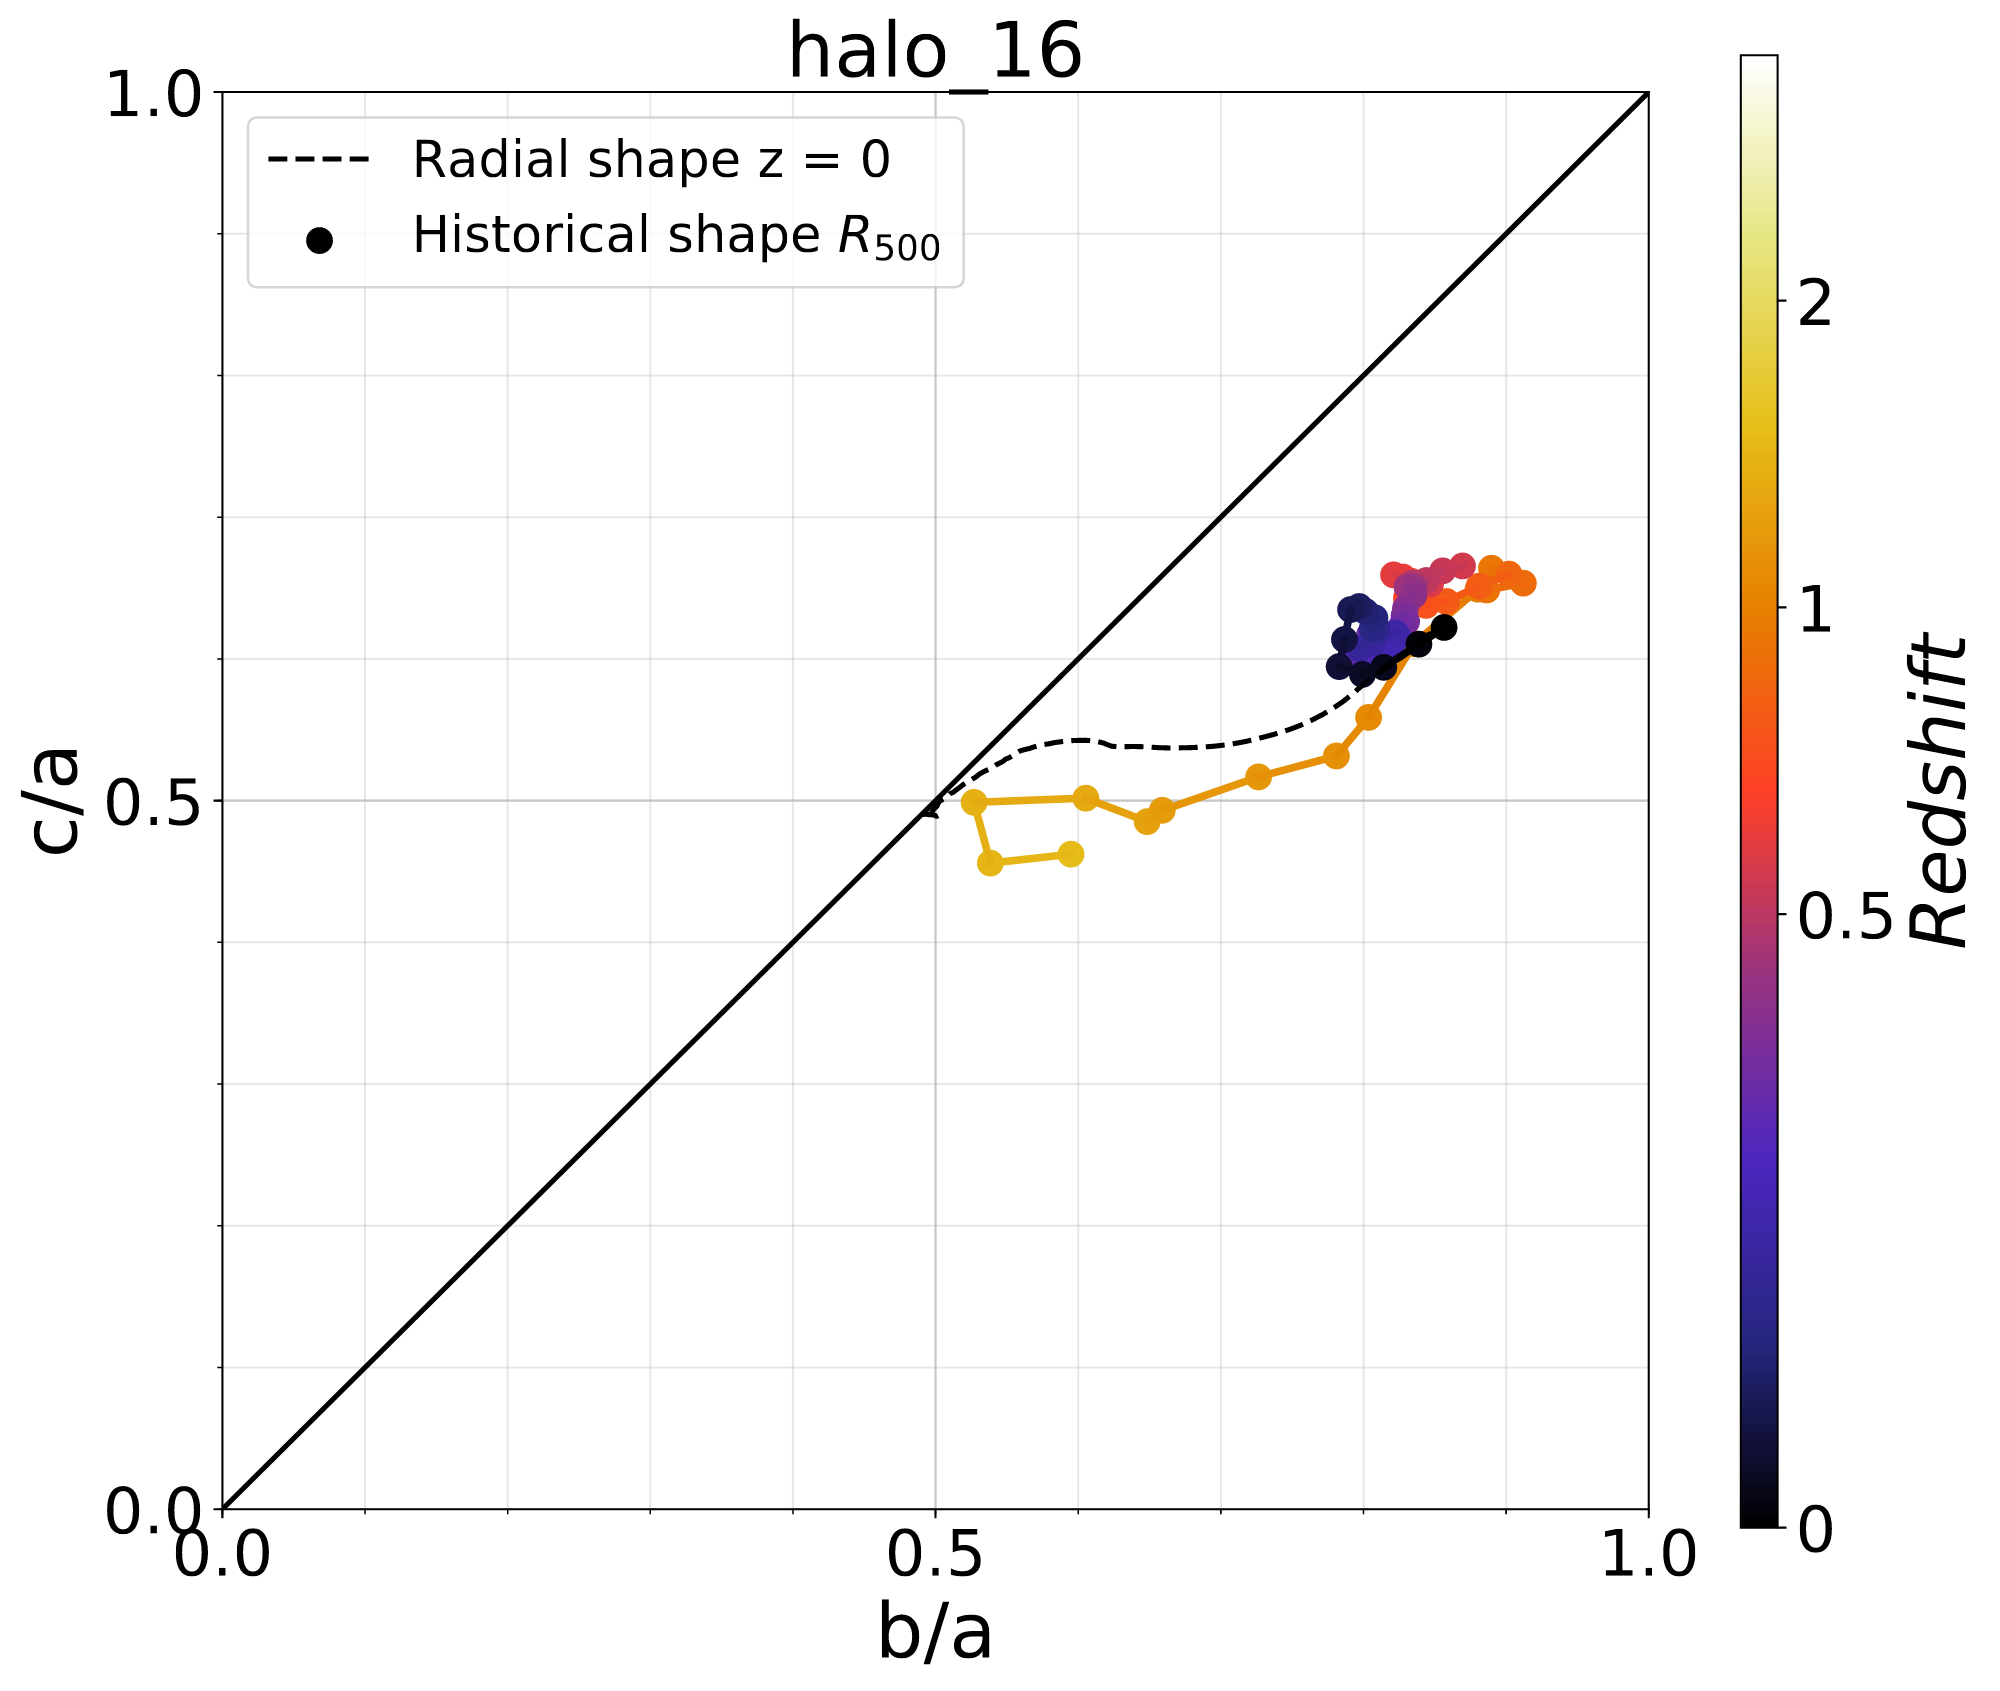
\includegraphics[width=0.5\columnwidth]{../Document/pics/Redshift/halo_16_level3_DM_Z_Triax.png}}
  \hfill
  \subfloat[\tiny halo 21 DM]{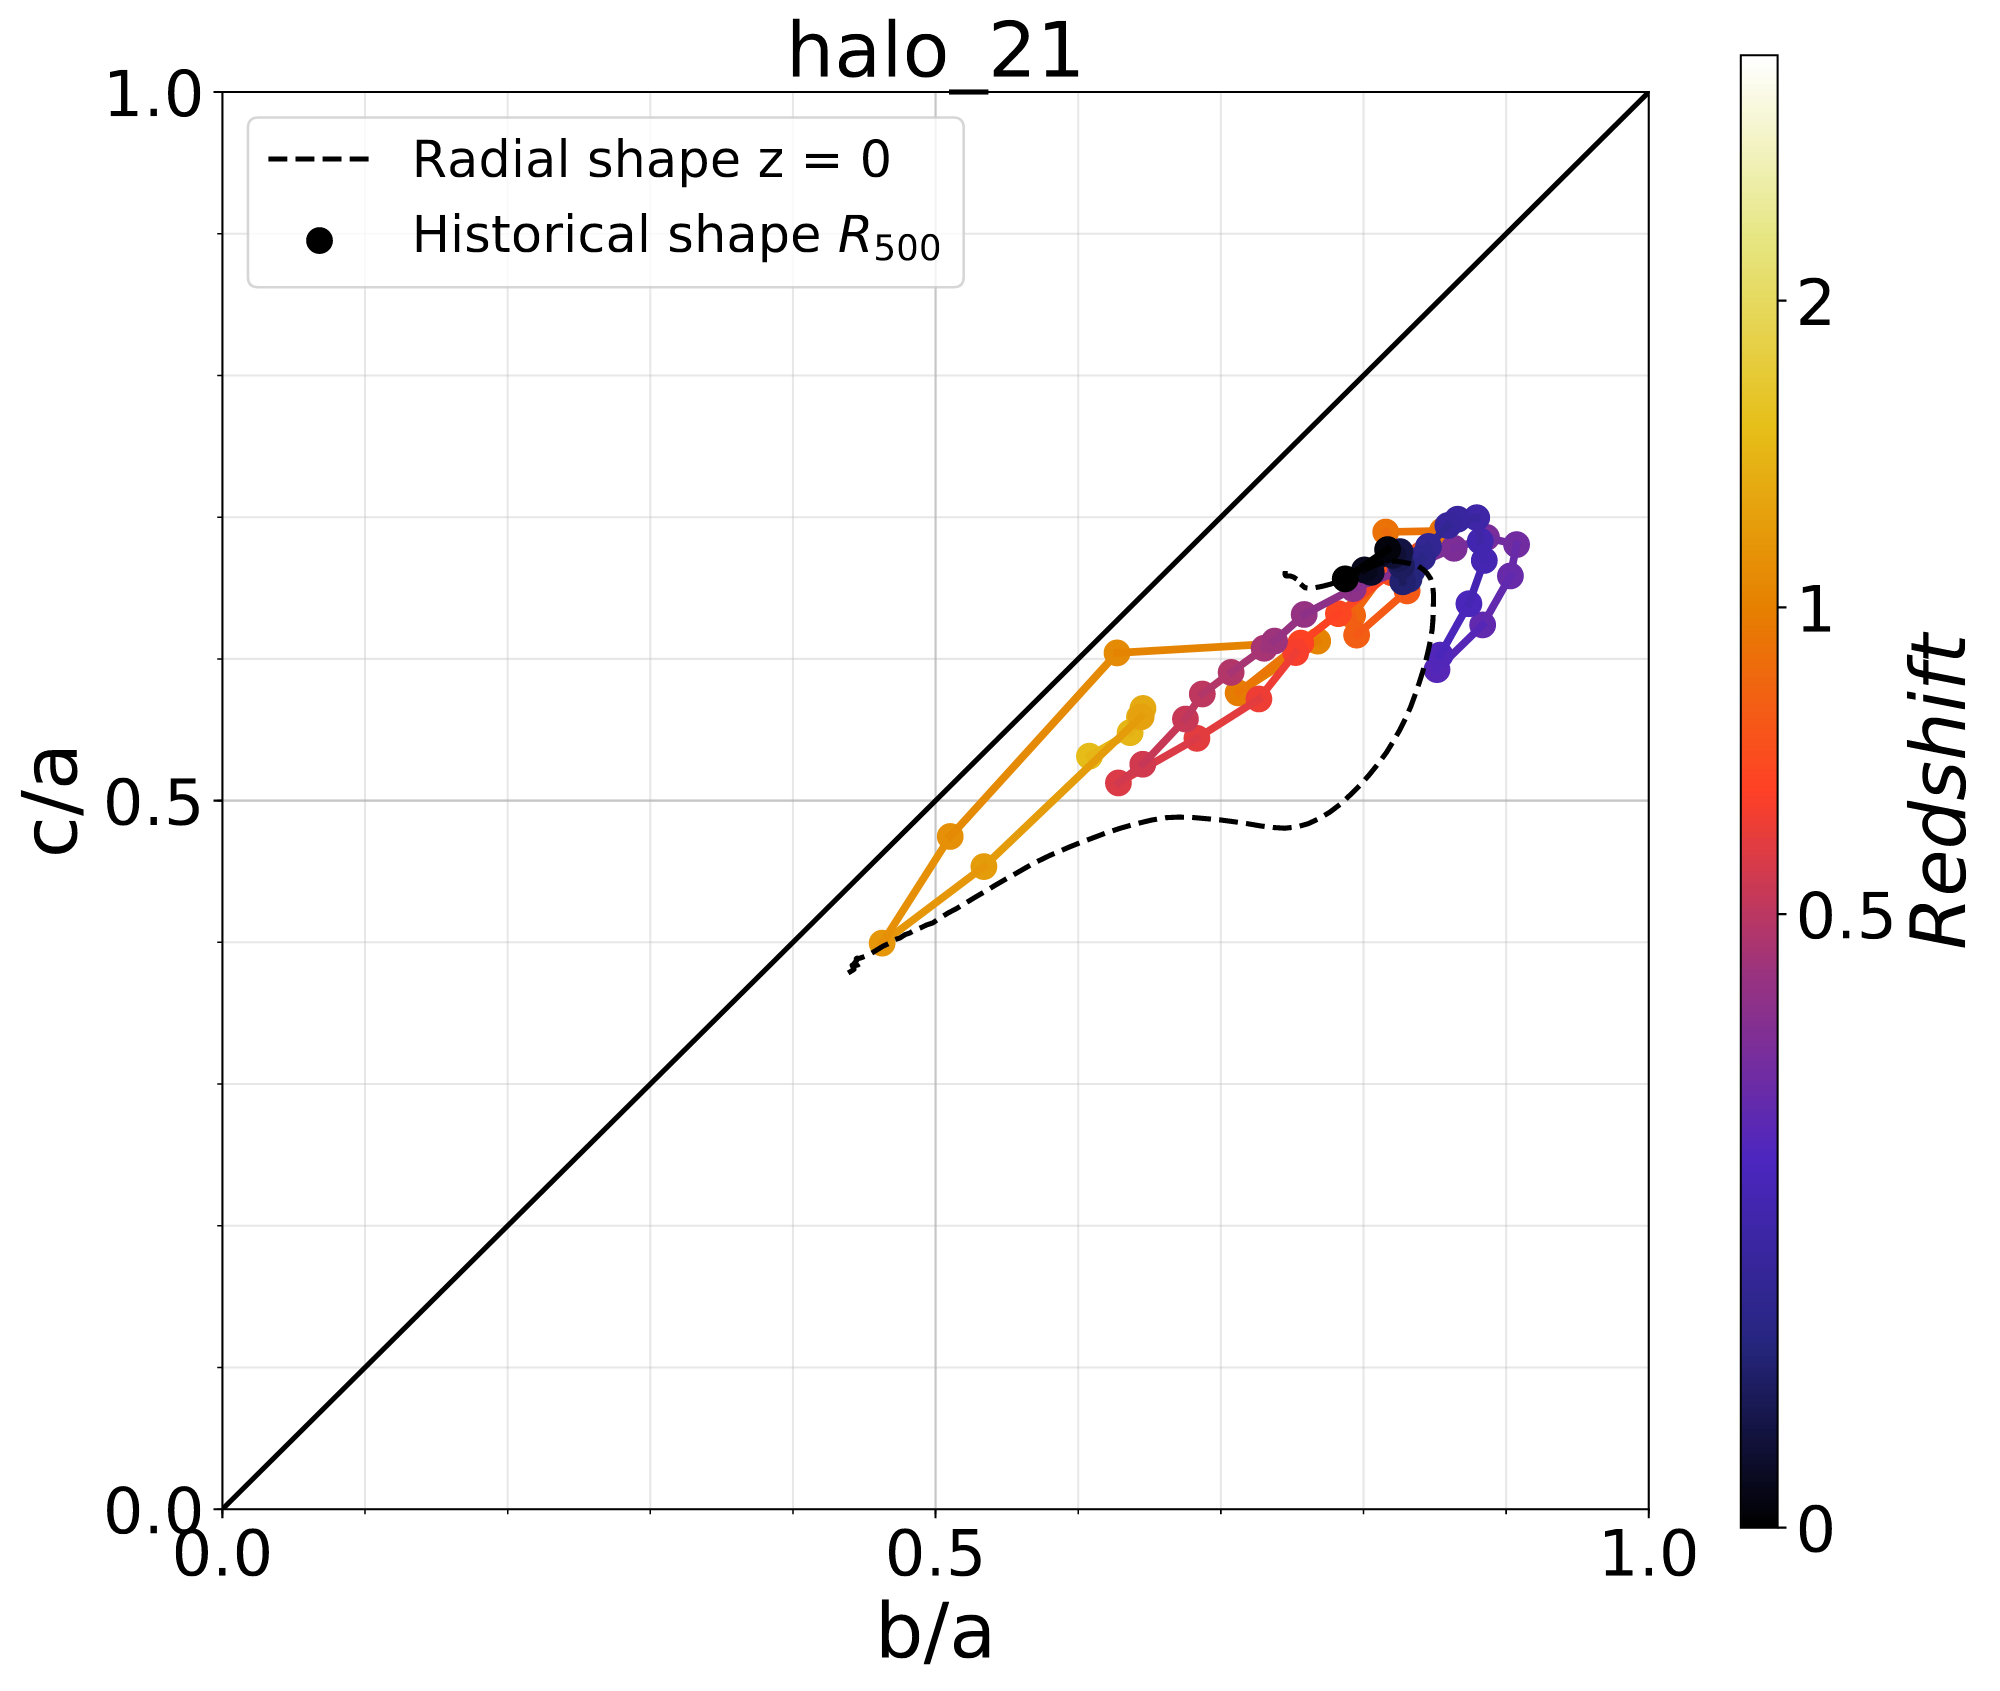
\includegraphics[width=0.5\columnwidth]{../Document/pics/Redshift/halo_21_level3_DM_Z_Triax.png}}
  %\caption{Historic shape (color dots) Vs actual radial shape (solid black line) on the Triaxiality plane. Each colored dot represents a calculated shape at R Mean 200, for each redshift. It is clear that halos with memory (halo 16), unlike disrupted halos (halo 21), have correlation between their historical and radial profiles.}
  \label{fig:RedshiftDM}
\end{figure}

\end{frame}


\begin{frame}[plain]
\begin{figure}[!ht]
  \centering
  \subfloat[halo 16 DM]{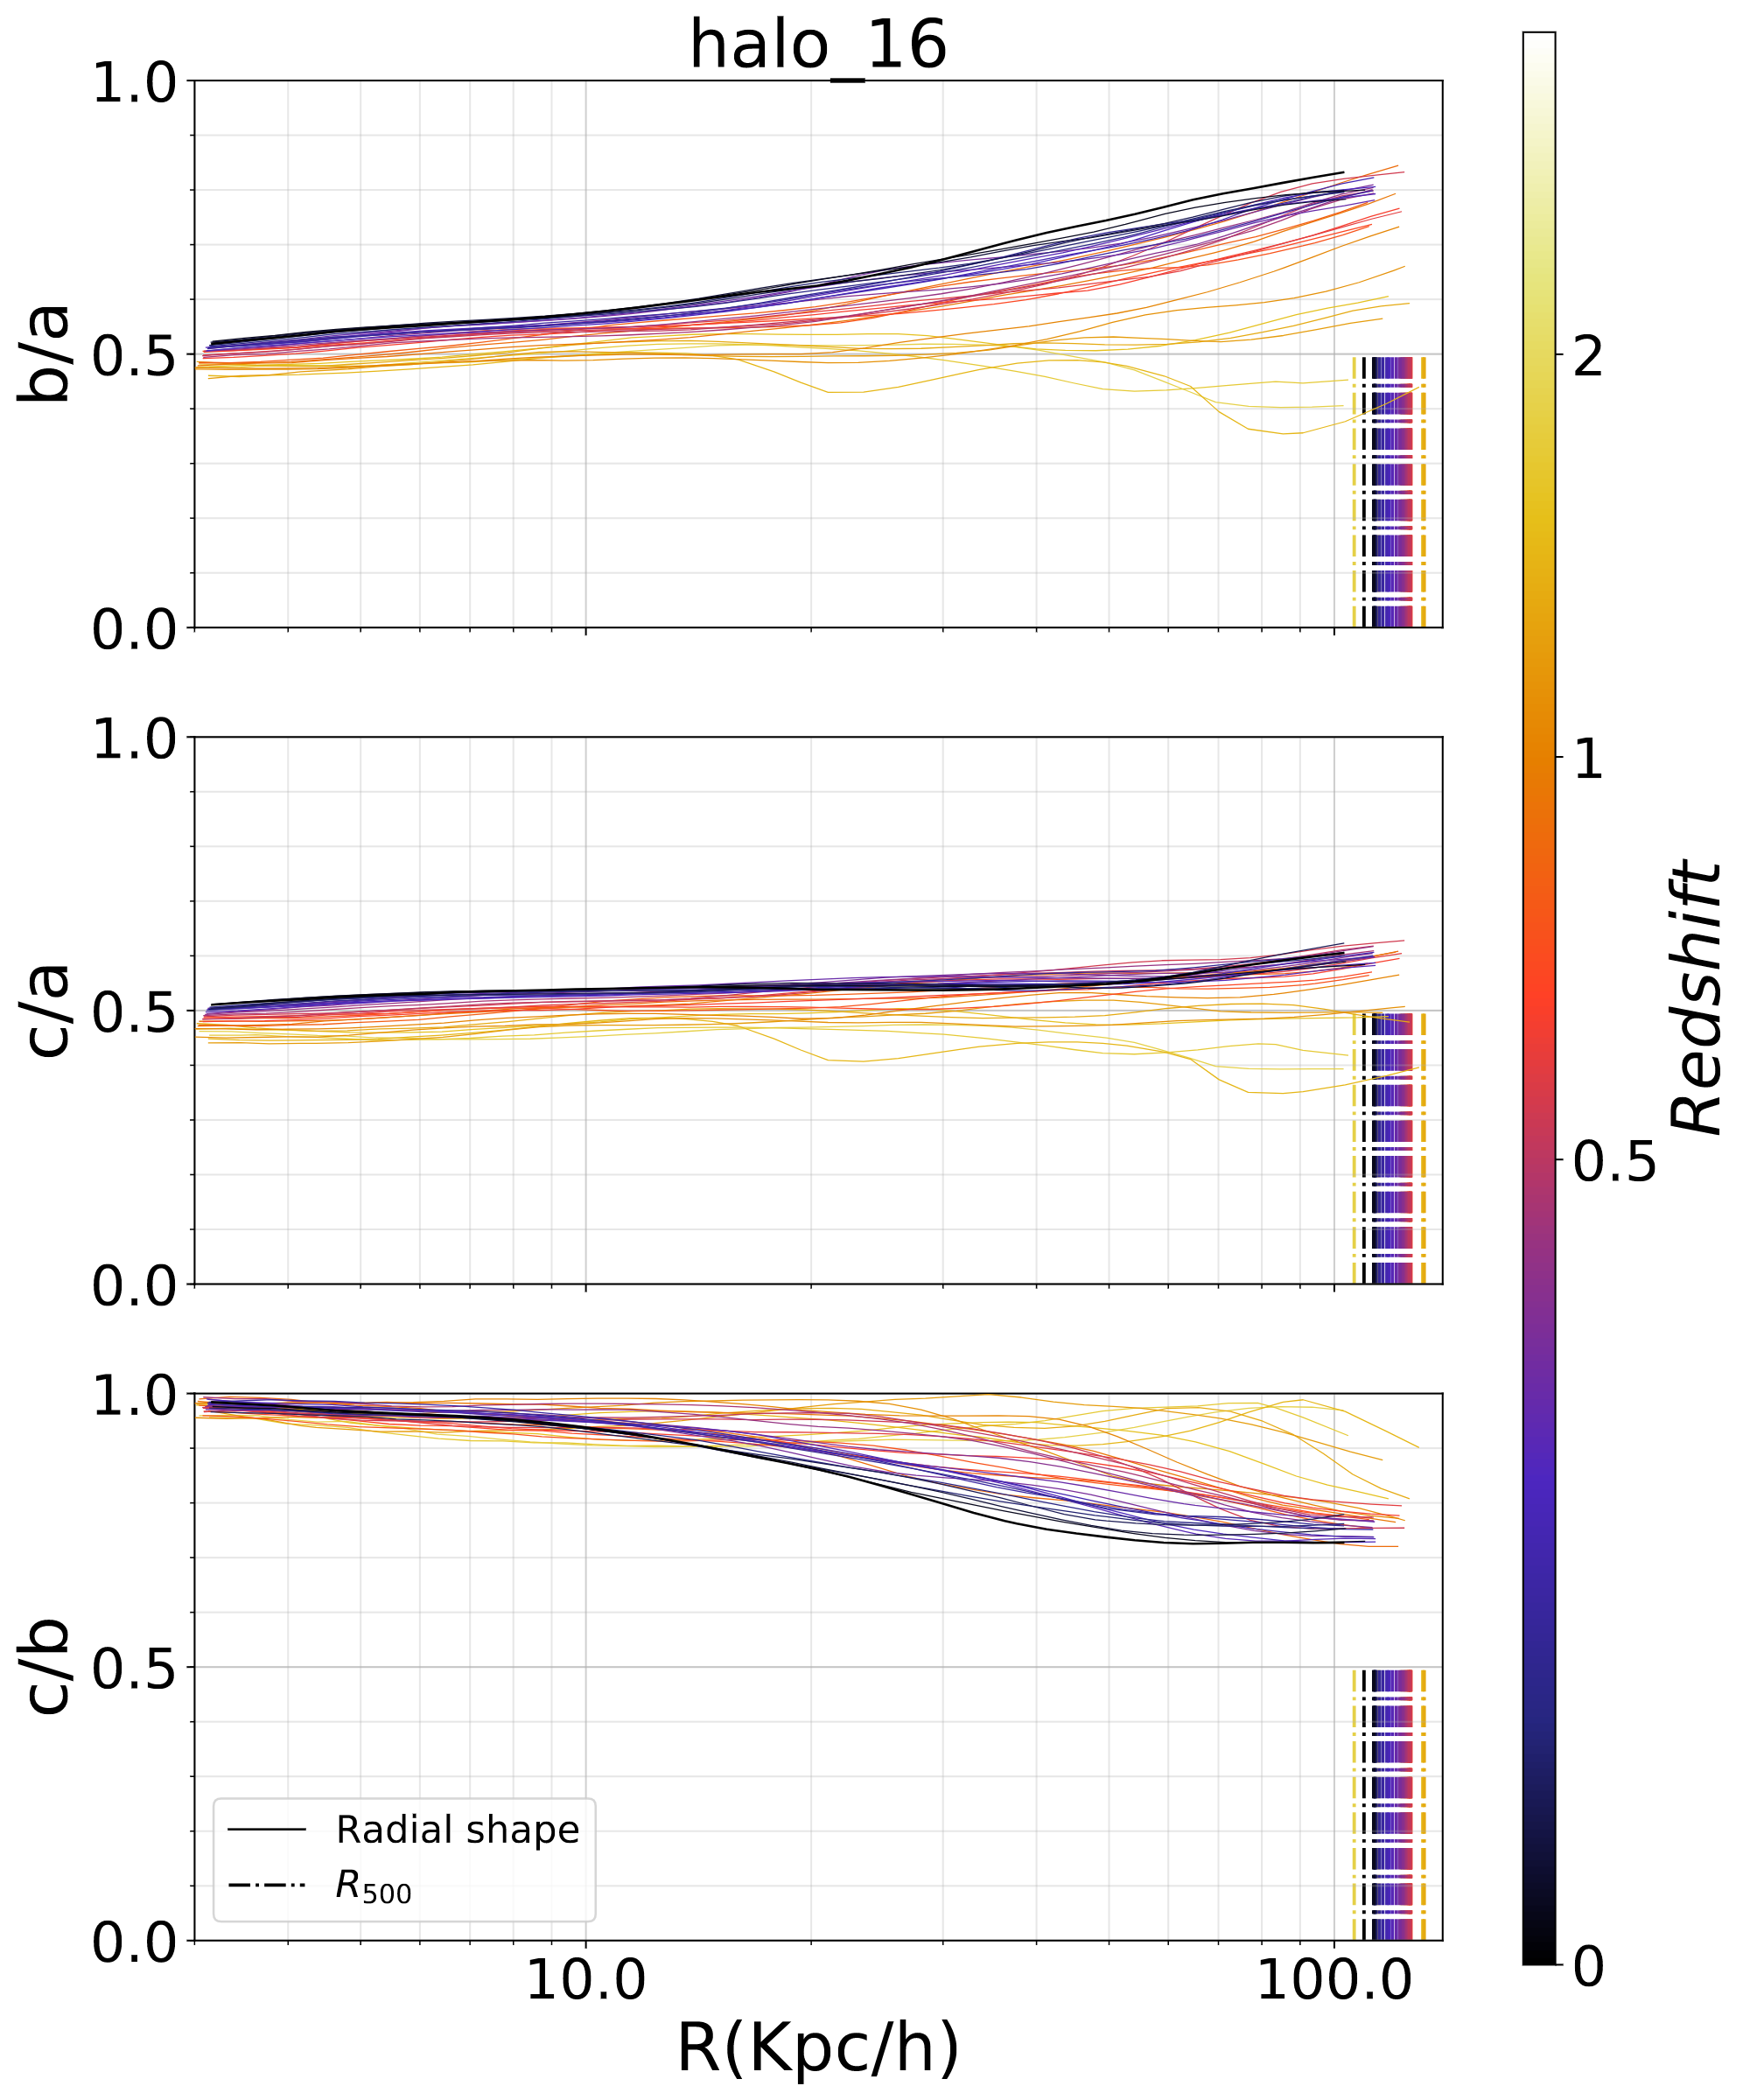
\includegraphics[width=0.45\columnwidth]{../Document/pics/Redshift/halo_16_level3_DM_Z.png}}
  \hfill
  \subfloat[halo 16 MHD]{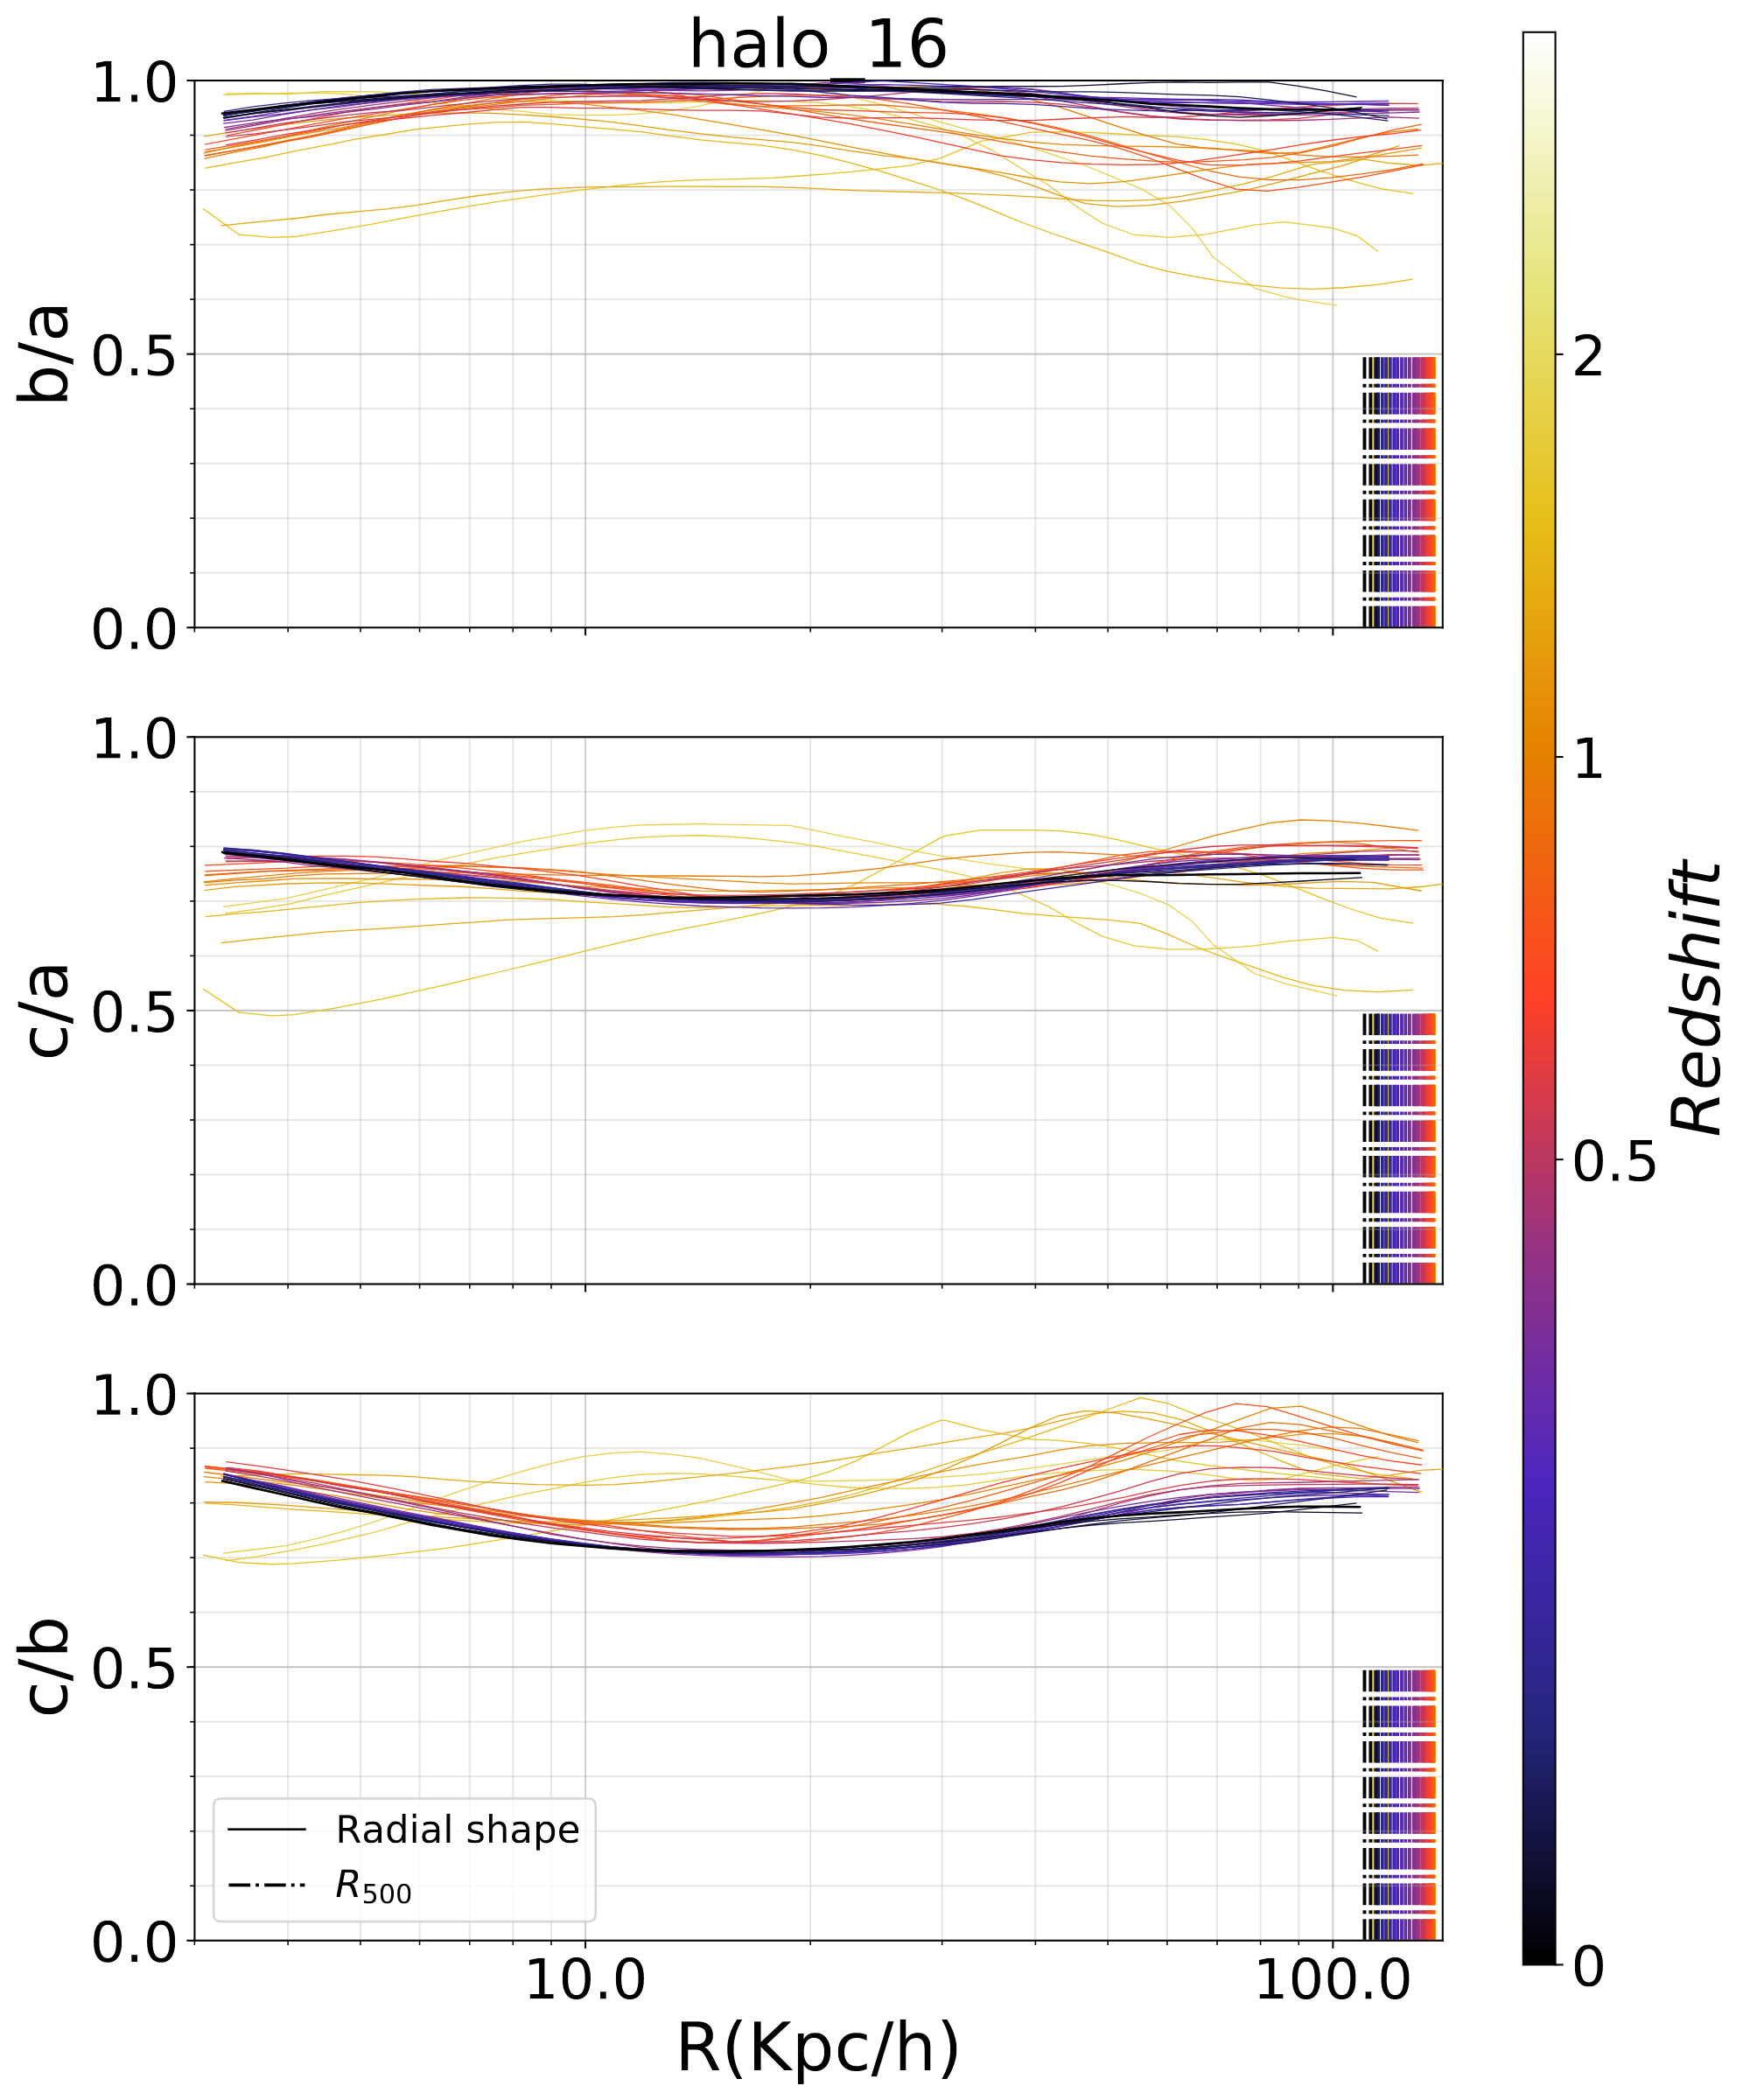
\includegraphics[width=0.45\columnwidth]{../Document/pics/Redshift/halo_16_level3_MHD_Z.png}}
  %\caption{Radial profile (comoving) of axial ratios for halo 16 in terms of redshift (color). This halo maintains its shape until $z\approx 1$ obviating the systematic rounding effect in time from asymmetric potentials. }
  \label{fig:RedshiftGood}
\end{figure}
\end{frame}


\begin{frame}[plain]
\begin{figure}[!ht]
  \centering
  \subfloat[halo 21 DM]{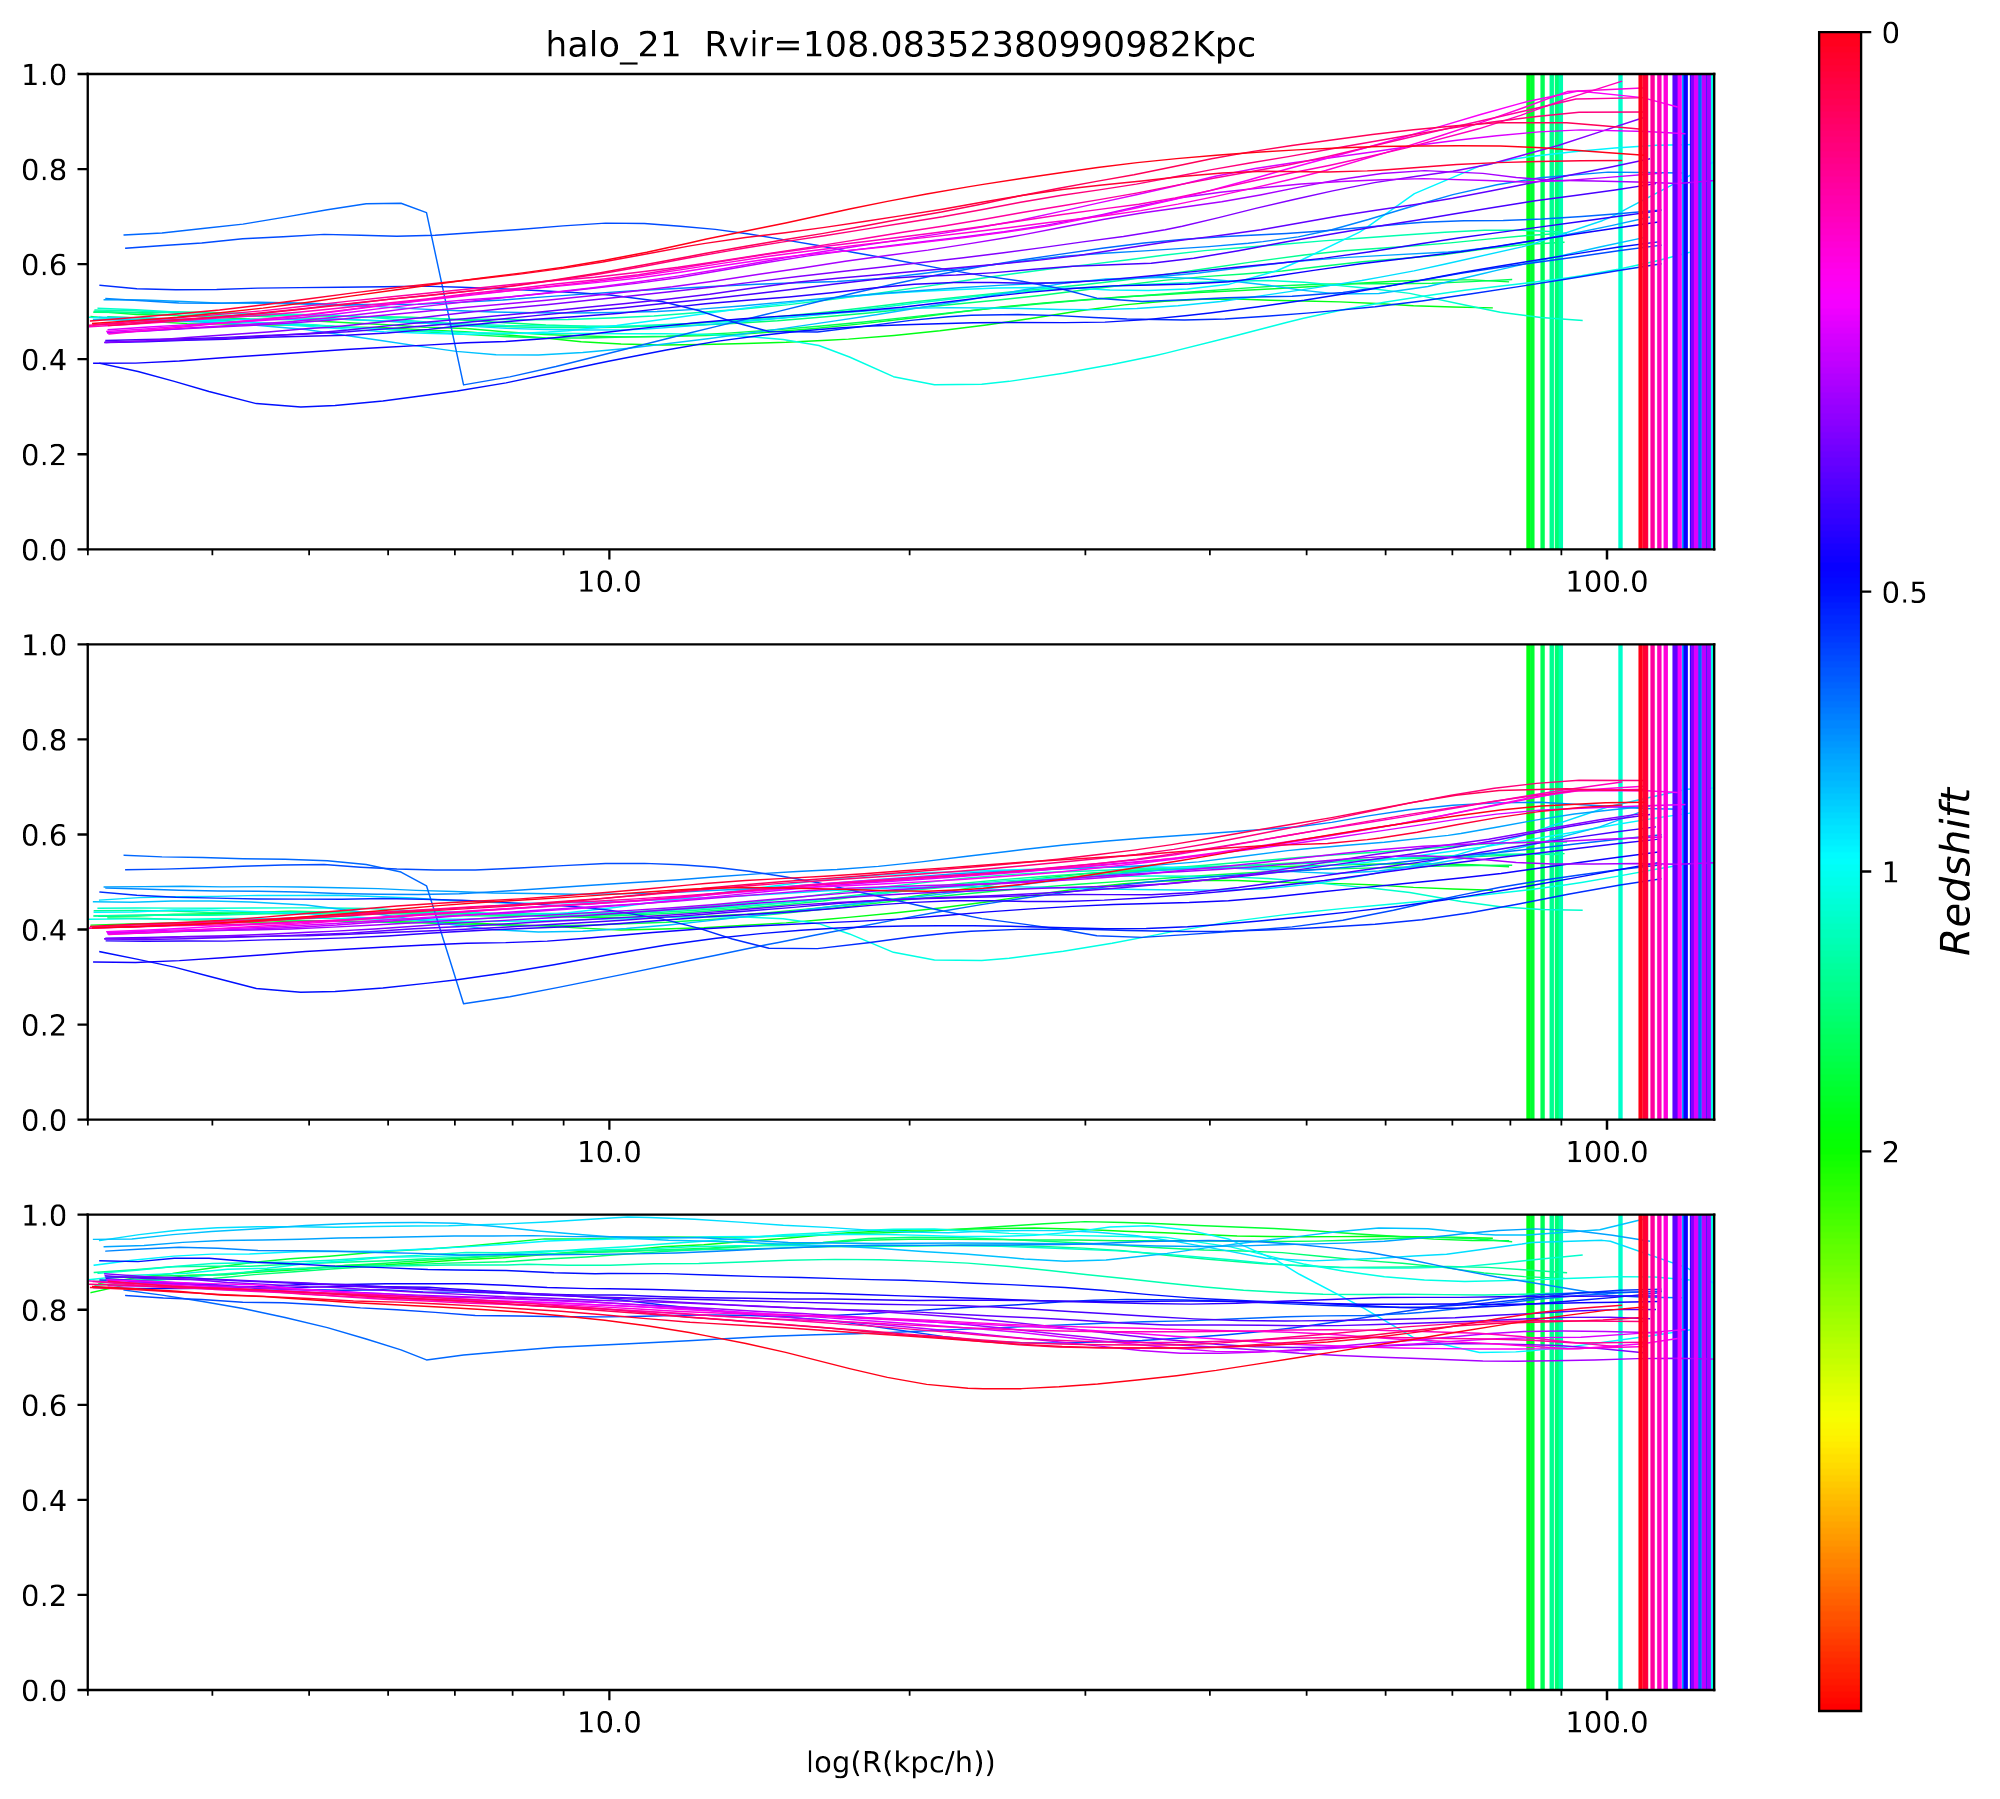
\includegraphics[width=0.45\columnwidth]{../Document/pics/Redshift/halo_21_level3_DM_Z.png}}
  \hfill
  \subfloat[halo 21 MHD]{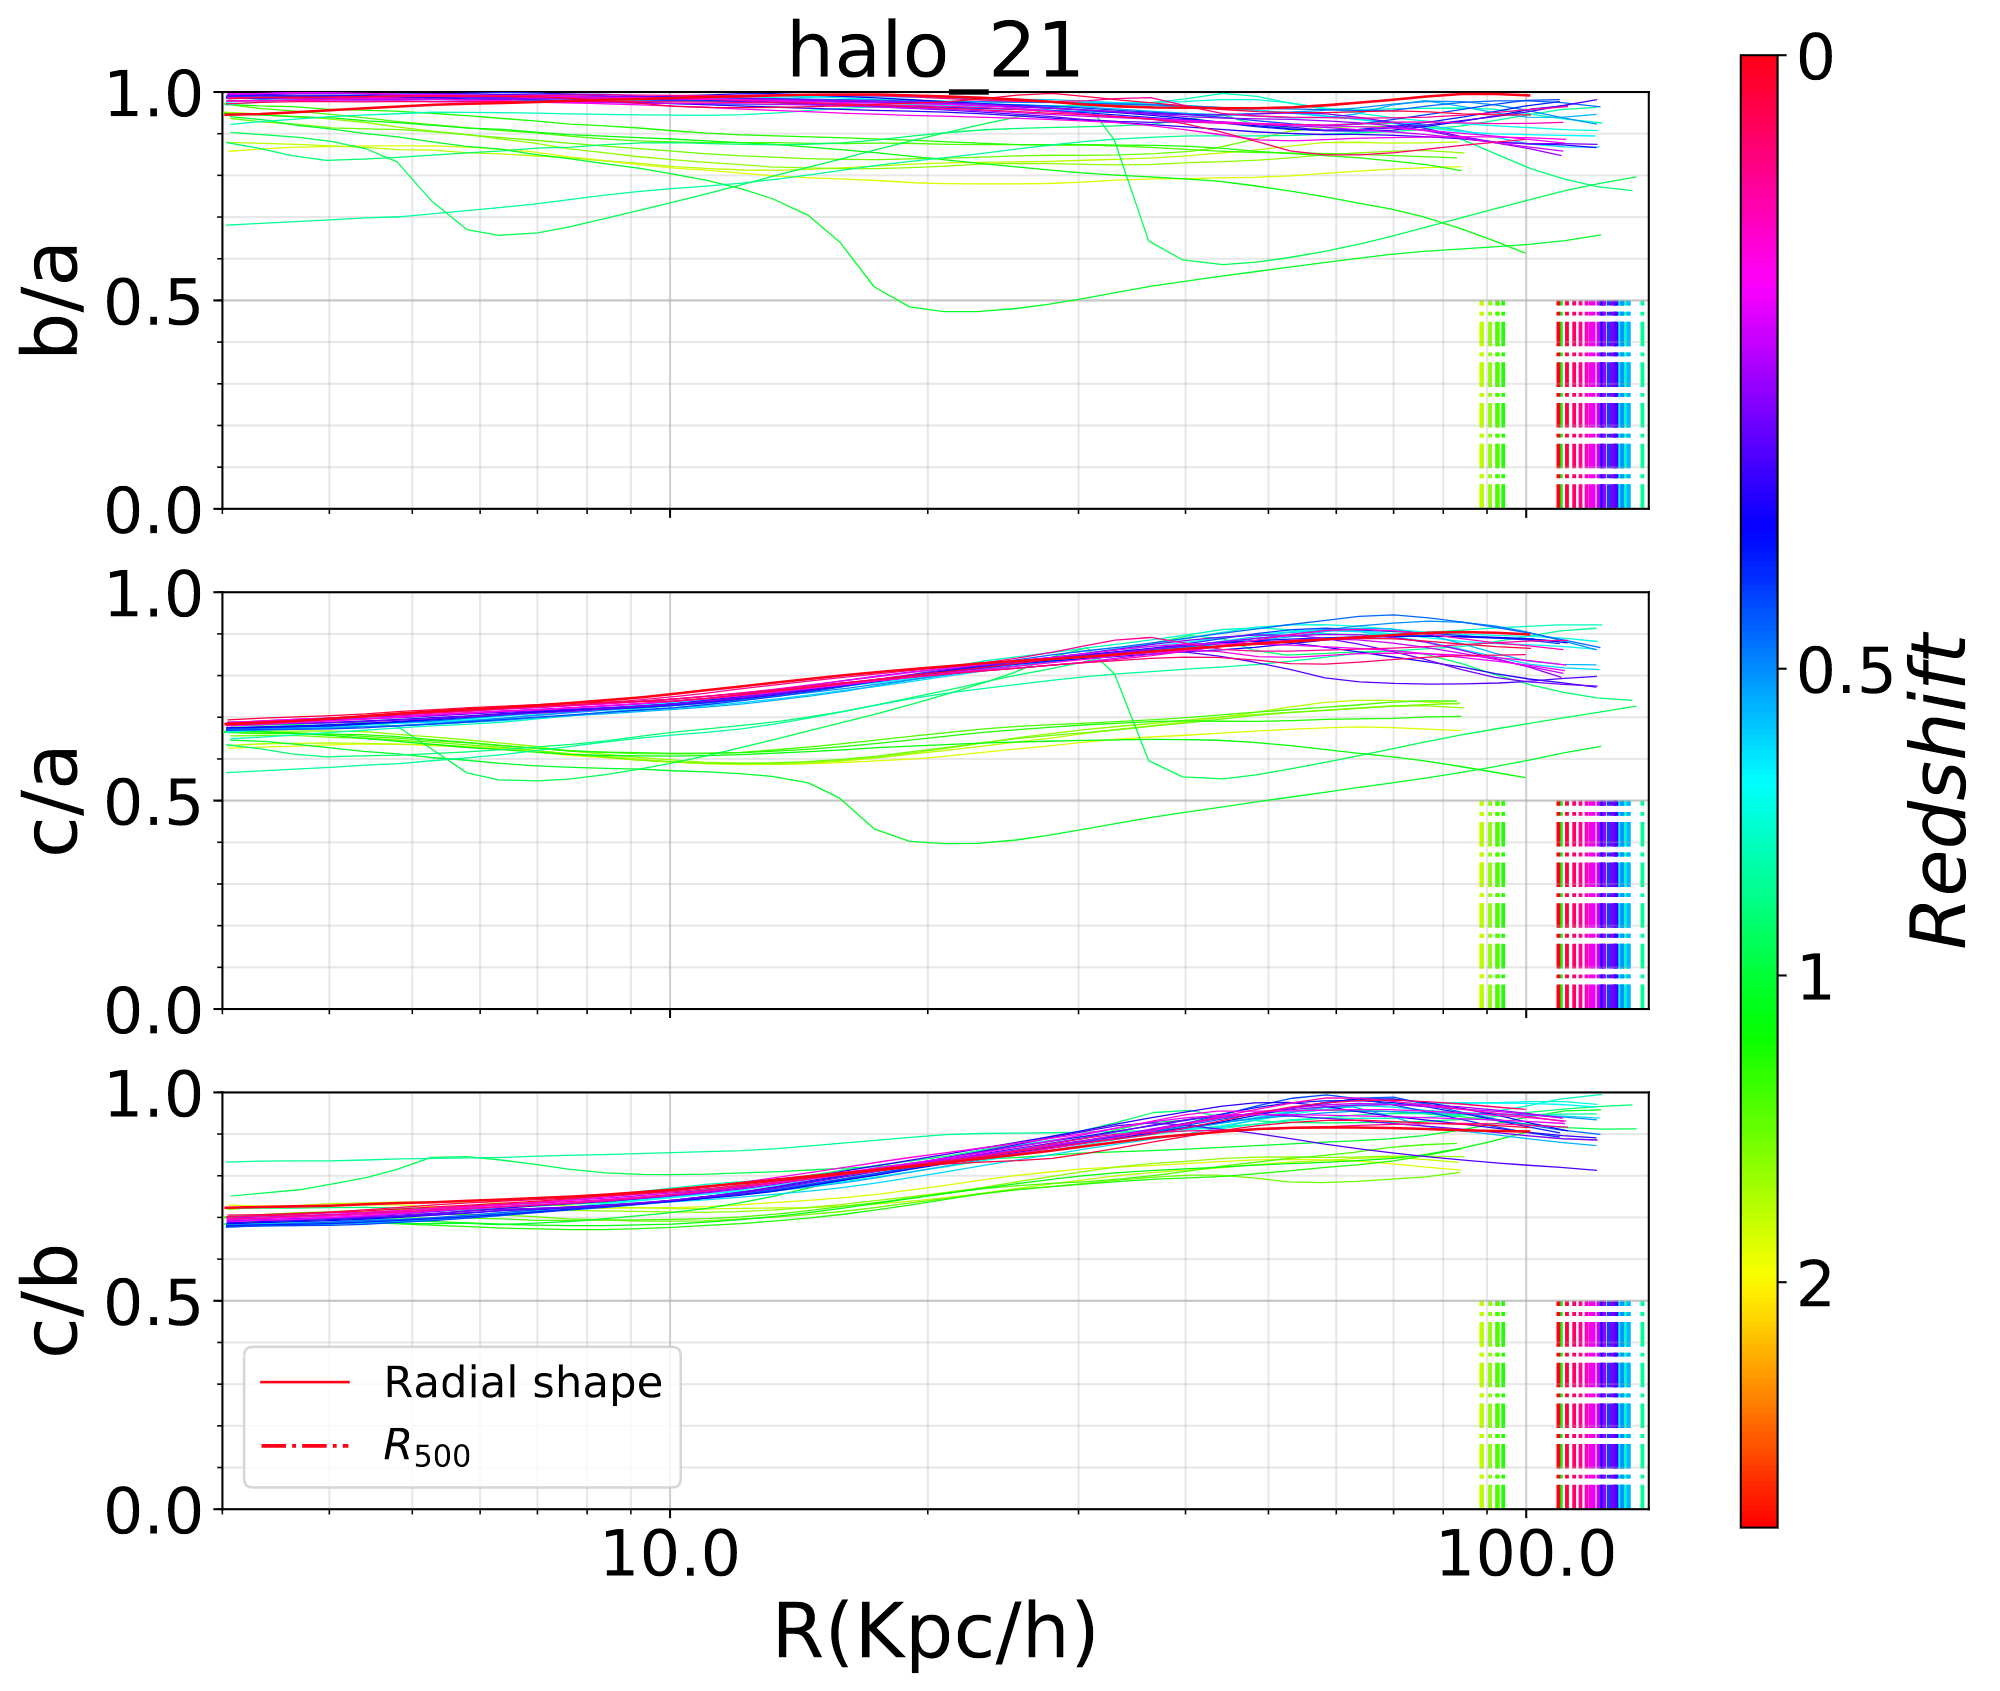
\includegraphics[width=0.45\columnwidth]{../Document/pics/Redshift/halo_21_level3_MHD_Z.png}}
  \caption{Radial profile (comoving) of axial ratios for halo 21 in terms of redshift (color). This halo is disrupted around $z \approx 0.5$ which results in a certain loss of its shape memory.}
  \label{fig:RedshiftBad}
\end{figure}


\end{frame}




%---------------------------------------------------------------------------------------
\section{Future work}

\begin{frame}

\begin{itemize}

\item Study the effec of environmental structures on halo shape and orientation.\\~\\

\item Study the response of DM halos to the presence of matter (Adiabatic contraction).\\~\\

\item Paper

\end{itemize}

\end{frame}

%---------------------------------------------------------------------------------------

%---------------------------------------------------------------------------------------


%---------------------------------------------------------------------------------------

%---------------------------------------------------------------------------------------


%---------------------------------------------------------------------------------------

%---------------------------------------------------------------------------------------



\section{References}
\begin{frame}[t, allowframebreaks]
\frametitle{Referencias}
\tiny
\bibliographystyle{unsrt}
\bibliography{Bibliography}
\end{frame}
\end{document}
